% select between bioRxiv style or submission style by commenting either line
%\documentclass[twocolumn]{bioRxiv}
\documentclass[submit]{bioRxiv}
\renewcommand\familydefault{\sfdefault}
\usepackage{lipsum}
\usepackage{enumitem}
\usepackage{placeins}
\usepackage{xcolor}
% authblk is loaded by bioRxiv.cls

% \usepackage[style=authoryear,backend=biber]{biblatex}
%% setup specific to this preprint -- add or remove as you need.
\hyphenation{empire} % prevents word "empire" being split across lines
\sisetup{range-units = single,
        uncertainty-mode = separate,
        separate-uncertainty-units = single,
        range-phrase = --} % units setup
\usepackage{multirow} % allows merging of cells in tables

% An unnumbered subsection that \nameref can point to (titlesec's starred sections do not record their title)
\makeatletter
\newcommand{\namedsubsection}[2]{\phantomsection\subsection*{#1}\def\@currentlabelname{#1}\label{#2}}
\makeatother

\begin{document}

%% comment out any files that you don't want to include as sections
\leadauthor{Bisot}
\title{Carbon supply for growth drives network-wide bidirectional flows in mycorrhizal fungi}

\shorttitle{Nutrient circulation in Mycorrhizal fungi}
\author[a,b,c,*]{Corentin Bisot}
\author[b,*]{Simon van Staalduine}
\author[b]{Achille Joliot}
\author[a,b]{Loreto Oyarte Galvez}
\author[d]{Filipe Henrique de Sousa Evangelista}
\author[a]{Marije van Son}
\author[d,f]{Howard A. Stone}
\author[a,e,f]{E. Toby Kiers}
\author[b,f]{Thomas S. Shimizu}

\affil[a]{Amsterdam Institute for Life and Environment, Vrije Universiteit, Amsterdam, The Netherlands}
\affil[b]{AMOLF Institute, Amsterdam, The Netherlands}
\affil[c]{European Molecular Biology Laboratory (EMBL), Heidelberg, Germany}
\affil[d]{Department of Mechanical and Aerospace Engineering, Princeton University, Princeton, NJ, United States of America}
\affil[e]{Society for the Protection of Underground Networks (SPUN), Dover, DE, United States of America}
\affil[*]{These authors contributed equally}
\affil[f]{co-corresponding authors}
\date{}
\maketitle

\begin{abstract}
 
Plant-mycorrhizal symbiosis is fundamental to terrestrial ecosystems as it is responsible for large flows of nutrients on a planetary scale. In this symbiosis, two distinct organisms trade phosphorus (P) for energy in the form of carbon (C). However, the mechanism behind the bidirectional transport of resources within their microscopic hyphae has not been entirely elucidated. We imaged transport dynamics of nutrient flows in high resolution in different positions in growing networks, and also perturbed flows through segment cuts and osmotic shocks. We find that carbon likely moves across the fungus on a directed network of molecular motor filaments. Our findings also suggest a tight coupling between network growth, internal carbon (lipid) transport dynamics, and bidirectional fluid movement within the network. The movement of lipids in the open pipe system inherently produces a backflow of cytoplasmic fluid, which may be responsible for the movement of phosphorus. Our model provides an intuitive understanding for the observed proportionality in resource exchange between the two organisms.
\end{abstract}

\section*{Introduction}
The symbiosis between Arbuscular Mycorrhizal (AM) fungi and their host plants has existed for 400 million years~\cite{remy_four_1994,brundrett_evolutionary_2018}. For the symbiosis to endure this long, robust mechanisms must be in place to ensure its stability. Indeed, symbiosis can be a many to many relationship, which means that the plant can interact with multiple independent fungal colonies and one fungal network can interact with multiple plant hosts~\cite{kiers_reciprocal_2011,walder_mycorrhizal_2012}. Without selective orientation of nutrients towards partners that engage in a proportional effort of nutrient provision, plant or fungal “free ride” phenotypes may emerge that reap the benefits of the symbiosis while avoiding costs~\cite{kiers_reciprocal_2011,bever_preferential_2009,walder_regulation_2015,noe_mycorrhizal_2018,kiers_misconceptions_2016}. 

The fungal partner forms a network in the soil using plant derived carbon. It absorbs phosphorus from the soil, which is then transported back to the plant. This means that carbon must constantly be shipped to the growing edge of the colony away from the plant, while phosphorus needs to be transported back in the other direction. Like other coenocytic fungi, AMF have aseptate hyphae, meaning that the organism can be considered a fully open pipe system, while they are growing. The mechanisms that could explain such bidirectional transport in a network of open pipes are so far unknown.

Our group had previously estimated that the fungal use of carbon for growth was proportional to the flux of phosphorus towards the plant~\cite{bisot_carbon-phosphorous_2025}, when a single AM fungus was attached to a single plant. In addition, it has been observed in the past that, when a single AM network was connected to two different plant hosts that differed in their carbon supply, more phosphorus was directed towards the plant that provided more carbon~\cite{kiers_reciprocal_2011}. 

Past research has quantified the flow speed in both directions in networks of different ages~\cite{oyarte_galvez_travelling-wave_2025}. However, without staining the lipids and/or phosphorus, it is difficult to understand the organization of resource flow across the network and the underpinning transport mechanisms. Resource specific staining can shed light on the distribution of resource flux within the network. For example, using Nile Red staining, it was found that lipid density varies along the hyphae, from about 24\% of the hyphal volume near the root to about 0.5\% at the front, and that lipid bodies move in both directions, mostly with the cytoplasmic stream~\cite{bago_translocation_2002}. A role for microtubule tracks in this movement has been proposed, but to our knowledge it has never been tested.

Flow speeds along the hyphae are modulated with time and location within the network~\cite{oyarte_galvez_travelling-wave_2025}. This can be interpreted through a traffic analogy inspired by the observed correlation between betweenness centrality, a typical transport network metric, and flow speeds. The betweenness centrality being the sum of times a shortest path between arbitrary nodes in a network crosses a particular network edge. Here, we set the root and tip nodes as the set of source and target nodes. However, this correlation lacks a direct physical basis that explains how such a relationship between global metrics and flows could emerge mechanically. Because AM fungi are coenocytic, the colony can be represented as a hydraulic network of connected pipes with varying radii. This hydraulic coupling between all elements of the network could generate spatial correlation in ways that can be physically framed. Such a mechanical framework, validated against measurements, for growing AM colonies is still missing.

What mechanisms explain the bidirectional transport of resources in the colony and its modulation over space and time? How can the transport mechanisms in place maintain a form of bidirectional transport in which the magnitudes of resource flux in opposite directions are maintained proportional? 
To answer these questions, we acquired image data at two different spatial and temporal resolutions to quantify the flow speed in specific edges of growing networks. At high spatial and temporal resolution, we acquired bright-field videos of transport dynamics within single hyphal edges over multiple days. Using Nile red, a neutral lipid-specific fluorescent dye, we also characterized and quantified the movement of carbon in the form of lipids along these same edges. At low spatial and temporal resolution, we obtained time-lapse images of growing networks that were transformed into their equivalent mathematical graph. In this way, we can relate the growth of the network with the measured flow speeds observed in the same network, allowing us to explain high-resolution observations both mechanistically and quantitatively. Additionally, a small number of perturbation experiments were performed to characterize each flow direction. From these data and findings, we construct a minimal model that explains the observed bidirectional transport of resources in the colony and its modulation over space and time.

\section*{Results}
\subsection*{Asymmetric bidirectional speeds}
Fungal networks grow through the extension of fungal tips away from the root of the host plant. Over time, these elongated hyphae develop into a branched mycelial structure. The network's topological context therefore varies along the length of a hypha. Close to a growing tip, the network is most tree-like: 40\% of the edges within 1~mm of a tip are bridges, that is, not part of any loop, against 11--14\% of the edges further than 2~mm from a tip (Fig.~\ref{fig:hyphal_profiling}A, inset). Moving away from the tip, more growing hyphae depend on the same runner hypha, and anastomosis (fusion between a hyphal tip and a hyphal segment) creates loops, which give many alternative paths from the tip towards the root~\cite{oyarte_galvez_travelling-wave_2025}.

\begin{figure}
    \centering
    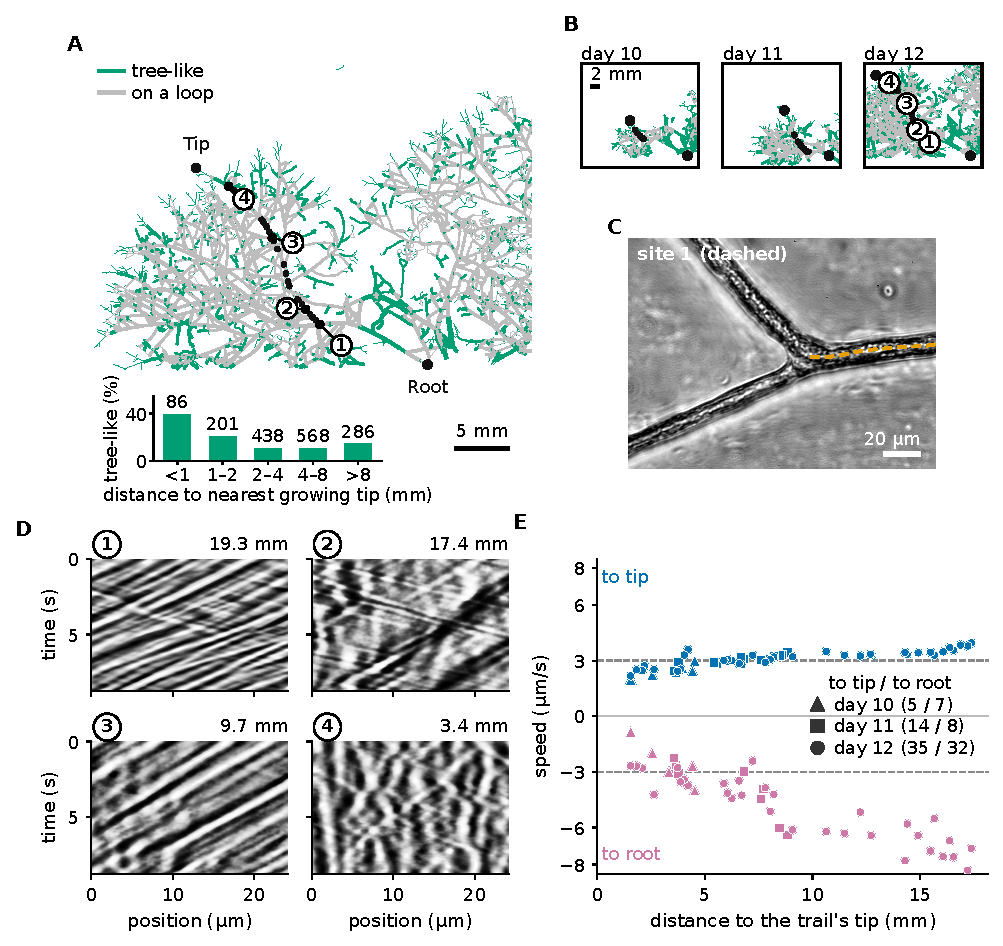
\includegraphics[width=\textwidth,height=0.72\textheight,keepaspectratio]{figures/Figure_1_v4.pdf} 
    \caption{\textbf{AMF produce robust patterns of asymmetric bi-directional flows across time and space.} \textbf{(A)} Network graph where a hyphal transect has been highlighted with dots where measurements took place. Green edges are tree-like, grey edges lie on a loop; line weight is exaggerated hyphal diameter. Inset: share of tree-like edges among the filmed edges (15 networks) by network distance to the nearest growing tip; numbers are edges per bin. \textbf{(B)} Time evolution of network across three days after the network started crossing into the fungal compartment. Dots indicate locations where videos were taken. \textbf{(C)} Example video frame of site 1, with edge indicated which is shown in D1. \textbf{(D1, 2, 3, 4)} Kymographs from respective locations in B, normalized by time-averaged value, and enhanced with CLAHE~\cite{pizerAdaptiveHistogramEqualization1987}. \textbf{(E)} Velocity profile along the trail shown in A, relative to the distance from the tip at the time of measurement. Each point is one video: the median of its extracted to-tip (blue) or to-root (pink) speeds. Marker shape gives the day, with the number of videos to tip / to root in the key; dashed lines mark $\pm 3~\mu m/s$.}\label{fig:hyphal_profiling}
\end{figure}

We asked how this change in topological context affected the speeds of the flows in the two directions along a hypha: towards the growing tip (to tip) and towards the root (to root), as defined by the growth direction of the network. We imaged flows at high resolution in 839 bright-field videos along the hyphae of five colonies (SI Fig.~\ref{fig:video_positions}) and, mostly at the same positions, in 704 videos of Nile Red fluorescence; for the example network of Fig.~\ref{fig:hyphal_profiling}, the videos were taken over three consecutive days. We chose runner hyphae, the main routes to the root and the edges of high betweenness centrality~\cite{kirkley_betweenness_2018}, where the to-tip and to-root flows could be told apart by eye. 

In undisturbed hyphae (SI section on lid-on lid-off paradigms), the two flows are superimposed in the video and move in straight lines at nearly constant speed, so that in a kymograph every moving particle leaves a straight diagonal streak, with no sign of random or back-and-forth movement (Fig.~\ref{fig:hyphal_profiling}D). Over the field of view, directed movement exceeds diffusion by more than two orders of magnitude, so the slope of a streak is its speed. Each streak gives one speed, and each kymograph was reduced to a set of to-tip and to-root speeds (SI Fig.~\ref{fig:speed_flux_extraction_real_data}).
% NOTE (6 Oct, answers Coco's 'why is there little diffusive movement?'): Peclet estimate, order of magnitude only. Assumed: lipid droplet 0.5 um diameter, cytoplasm viscosity 10x water (0.01 Pa s), T 295 K: D = kT/(6 pi eta r) = 0.09 um^2/s; over a 10 s kymograph sqrt(2Dt) = 1.3 um against 30 um at 3 um/s; Pe = vL/D with L = 10 um = 350. Check the droplet size and viscosity before submission. Weaker near the tips (Fig 1D kymograph 4): issue #5.
In the histogram of the extracted speeds of a video, the to-tip speeds (positive) and the to-root speeds (negative) each form a peak. We took the median of each of the two groups as the speed of that direction in that video (Fig.~\ref{fig:hyphal_profiling}E). 
Speeds to tip slow down close to the tip, but stay close to 3~$\mu m / s$ further away (Fig.~\ref{fig:hyphal_profiling}E). Speeds to root increase with distance from the tip (Fig.~\ref{fig:hyphal_profiling}E), and have a wide range: the median interquartile range of a hypha's speeds is 1.6~$\mu m / s$ to root, against 0.6~$\mu m / s$ to tip (SI Fig.~\ref{fig:speed_iqr}). This result was confirmed by repeating a similar experiment over 33 repetitions showing a consistent phenomenology (Fig.~\ref{fig:asymmetries} A, B). 

\begin{figure}
 \centering
 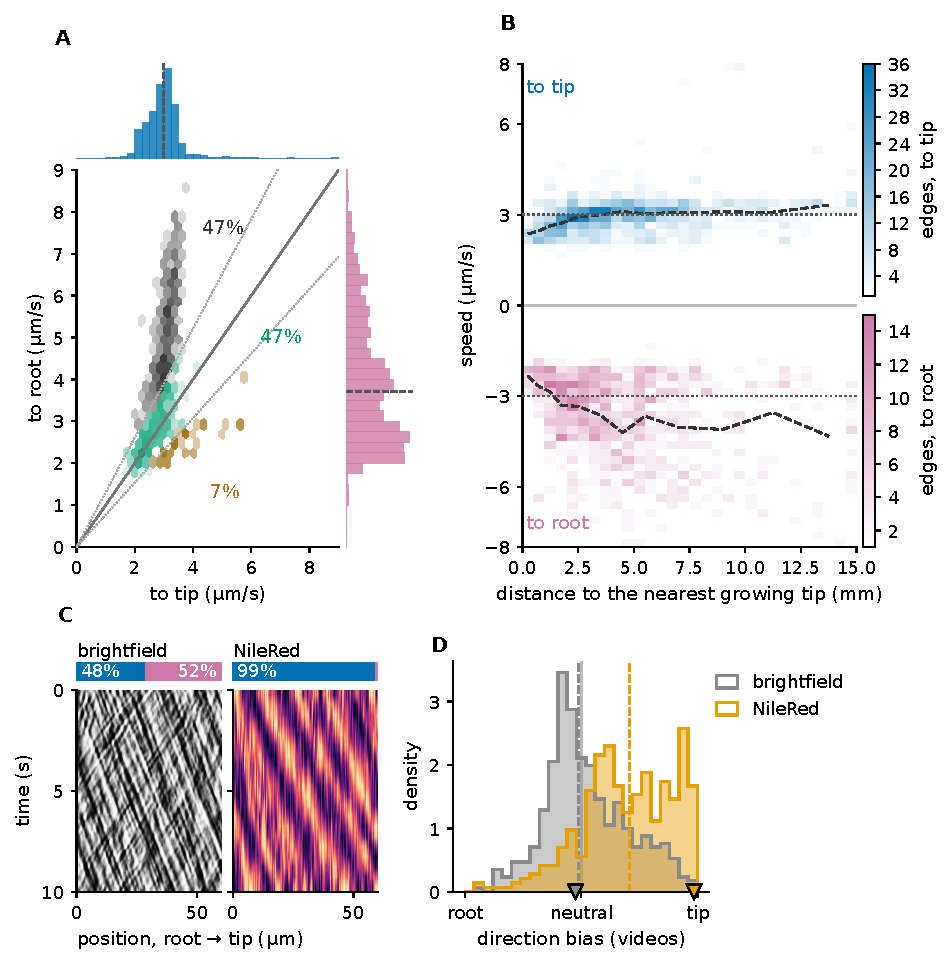
\includegraphics[width=\textwidth]{figures/Figure_2_v2.pdf}
 \caption{\textbf{To-tip and to-root flows differ in speed and in cargo: the to-tip flow is concentrated around $3 ~\mu m /s$ and carries most of the lipid, the to-root flow is more variable.} \textbf{(A)} Density of the absolute to-tip speed against the absolute to-root speed at the same location, in bright-field. Marginal histograms along the edges. Hexagons are coloured by their ratio to 1:1 within a factor 1.3: to-root faster (black), similar (green) or to-tip faster (orange); percentages give the share of the data in each class. \textbf{(B)} Density of the measured speeds against the distance to the nearest growing tip: to tip (blue) and to root (pink), with the median per column (dashed) and $\pm 3 ~\mu m/s$ (dotted). \textbf{(C)} The same position imaged in bright-field (left) and Nile Red fluorescence (right), 15 seconds apart; bars give the share of the speed-weighted moving signal going to the tip (blue) and to the root (pink). \textbf{(D)} Direction bias per video, the share of the speed-weighted moving signal going to the tip (median over the edges of the video; videos with too little directed signal left out), from bright-field (grey) and Nile Red fluorescence (yellow). Dashed lines: medians; triangles: the example shown in C.}\label{fig:asymmetries}
\end{figure}

We asked if the asymmetry in the directional speeds could be due to the difference in cell components that would be moving in the two directions, which could inform the mechanism of movement. We stained neutral lipids with Nile Red fluorescent dye~\cite{bago_tracking_2002} and imaged the same positions with both bright-field and fluorescence setups (Fig.~\ref{fig:asymmetries}C, D). At the resolution of the fluorescence videos (0.14~$\mu$m per pixel, 0.5 or 1~s per frame, 10 to 20~s per video), we saw no evidence of lipid particles randomly switching direction, as they would in the random walk underlying diffusive motion (Fig.~\ref{fig:asymmetries}C). The lipids moved to the tip at a median of 2.15~$\mu m/s$ (879 edges with both directions measured in fluorescence), somewhat slower than the 2.95~$\mu m/s$ of the bright-field to-tip stream (SI Fig.~\ref{fig:fl_forward_backward}). In the other direction, fewer fluorescence streams were detected (989 against 1,396 to tip), at a median of 1.96~$\mu m/s$ against 3.55~$\mu m/s$ in bright-field. These fluorescence speeds are limited from above: the fluorescence videos have only 10 or 20 frames (bright-field 200), and the detection of a streak falls steadily with its speed, to about a fifth of its slow-speed level at 5--6~$\mu m/s$ at 2 frames per second, so fluorescence speeds above about 5~$\mu m/s$ are censored, not absent (Methods, \nameref{subsec:fl_detection_limit}). Speeds taken from the orientation of all moving pixels, which do not depend on the streak detection and follow the true speed up to 8 to 9~$\mu m/s$ at 2 frames per second, still show a smaller to-root branch in fluorescence than in bright-field: the to-root stream is faster than the to-tip stream by more than the 1.3-fold margin on 20\% of the fluorescence edges against 39\% of the same edges in bright-field (532 edges with both measured). So the detection limit explains part of the lower fluorescence speeds in the to-root direction, but not all of them, and why the stained cargo returns more slowly than the bright-field backflow remains open (Methods, \nameref{subsec:fl_detection_limit}).
% In general, lipid velocities agree with what is measured in bright-field, with the exception of some tip-to-root videos, where they appear to go slower than the measured speed in bright-field (Fig \ref{fig:hyphal_profiling}e). 
By comparing bright-field and fluorescence videos of the same position, recorded about 15 seconds apart, it is clear that only a subset of trails visible in bright-field kymographs appear also in the fluorescence version (Fig.~\ref{fig:asymmetries}C, D): fluorescence gives 625 videos and 879 edges with both directions measured, bright-field 731 videos and 1,513 edges. We set out to find whether there was a directional bias in the movement of lipids. For each video we computed the share of the moving signal that travels towards the tip, from 0 (all to the root) to 1 (all to the tip) (Methods, \nameref{subsec:direction_bias}). Together, these results show that lipids generally move in the direction of the tips (Fig.~\ref{fig:asymmetries}D). 

% We wanted to know how general the observation was that the speeds observed in the network were asymmetrically distributed over the two possible directions. In order to assign a direction to each edge of the network, we used the lipid flux direction that we could determine from the fluorescence video. We associated one speed with the speed of particles moving in the same direction as the lipid flux, and the other to the particles moving in the other direction. This procedure was performed on the whole dataset comprising 6 developmental timepoints from 2 different plates and a total of $\sim$ 2000 edges (SI Fig.\ref{fig:replicates}). We found that the distribution of particle speeds moving in the lipid direction was narrow and peaked around a value of $3\mu m/s$ (Fig. \ref{fig:hyphal_profiling}f). The speed distribution in the other direction was wider with a long tail at higher speed going up to $\sim 8\mu m/s$.

\subsection*{Perturbations show that cytoplasmic flow toward the root is pressure driven while lipids are translocated by molecular motors}
\begin{figure} 
\centering
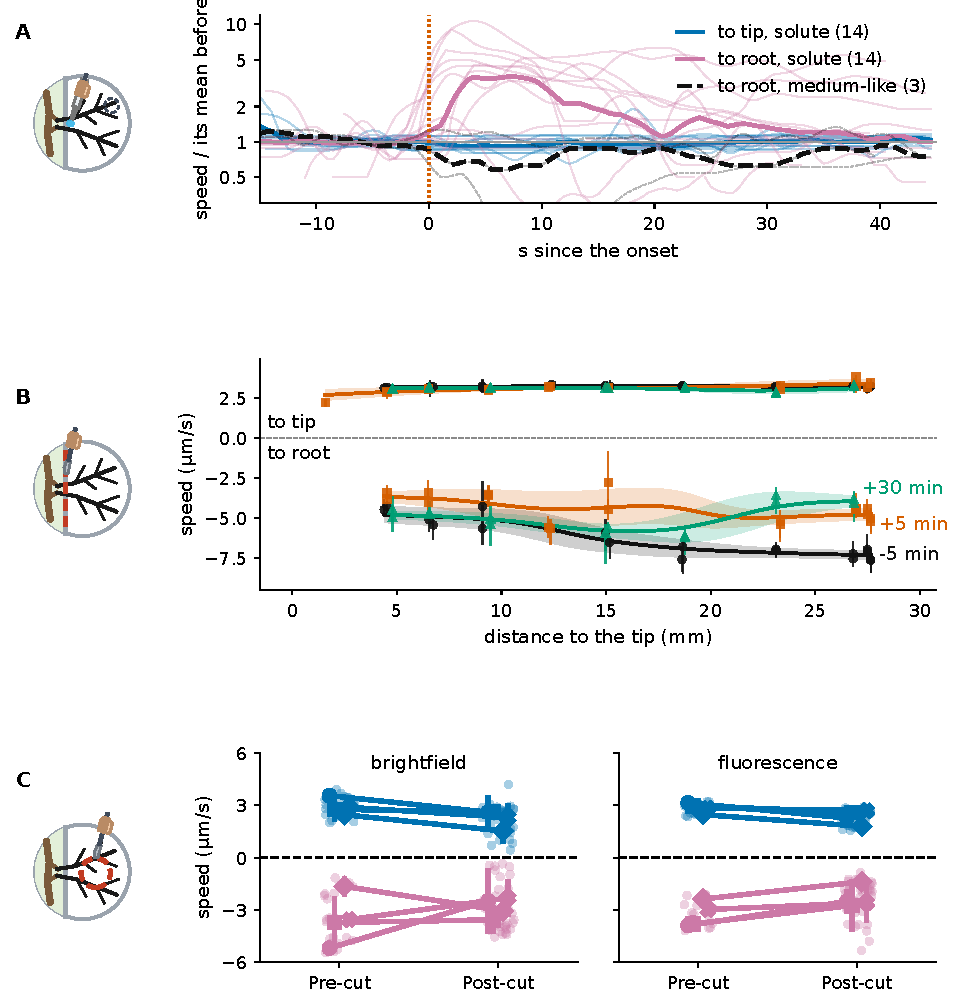
\includegraphics[width=\textwidth]{figures/Figure_3_v2.pdf} 
\caption{\textbf{Flows are driven by local elements, with limited whole-network influence.} \textbf{(A)} Osmotic shock: a drop of solute solution (mostly NaCl, 100 to 400 mOsm) placed on the substrate at the base of the network, a few centimeters behind the growing front, while a hypha near the growth edge is imaged. Speed divided by its mean before the drop, to tip (blue) and to root (pink): thin lines are single droplets, thick lines the median of the 14 solute droplets; the black dashed line is the median to-root speed of 3 medium-like control drops. Dotted line: onset of the response. \textbf{(B)} Root cut: the network is severed from the root along its whole bottom. Speed along a runner hypha against the distance to the tip, 5 min before (black), 5 min after (orange) and 30 min after (green) the cut. Positive speeds are to tip, negative to root. Points are positions along the hypha (bars: interquartile range of the videos), curves the kernel-averaged mean and shading $\pm 1$ standard deviation. \textbf{(C)} Section cut: a sub-graph of the network is isolated by cutting its connections (red lines in the icon). Speed before and after the cut in bright-field and in Nile Red fluorescence, to tip (blue, positive) and to root (pink, negative). Each marker shape is one isolation experiment: large symbols are the mean over positions in the segment, vertical bars the standard deviation, small dots the single videos. Pre-cut data were acquired at most 30 min before the cut, post-cut data from 30 min to 3 hours after it.}\label{fig:perturbations}
\end{figure}

In the past, pressure gradients and molecular motors have been suggested to be potential mechanisms driving flows in fungal hyphae~\cite{heaton_growth-induced_2010,lew_mass_2005}. An ideal experiment to distinguish these two potential drivers would be to modify the pressure gradient across the network and see how it affects flows. This experiment has been done in the past by creating an extracellular osmotic gradient~\cite{lew_mass_2005}. Following a similar approach, we added a drop of dissolved NaCl solution (100 to 400 mOsm) (Reference to Methods SI) to the base of the network a few centimeters behind the growing front and imaged near the growth edge (Fig.~\ref{fig:perturbations}A). We expected that this would create a low turgor pressure within the hyphae at the location of the drop, shifting the pressure gradient within the network, and therefore changing flows internal to the hyphae. We observed that the flow speed in the tip direction was almost unaffected by the addition of the salt solution  (Fig.~\ref{fig:perturbations}A);  fluorescence imaging of the lipids showed that their movement in the tip direction was also unaffected (SI Fig.~\ref{fig:salt_shock}D). By contrast, the flow speed in the root direction was approximately raised to 3.5x and relaxed within a minute. Control drops had no effect, medium-like drops resulted in light hypo-osmotic shocks. 
% NOTE (2 Oct, NaCl concentration): droplet series = 14 solute droplets at 100-400 mOsm (mostly NaCl; example movie NaCl 100 mM; one sucrose 50 mOsm) + 3 medium-like controls (transport_paper salt_shock_relax.py, Fig S salt shock). Give the range or the one shown.

The difference in flow behavior both within an edge, and along an edge with distance to tip, suggests that each direction could be associated with a different mechanism. Past work proposed that plant host transpiration could be the driving force explaining the flow of resources towards the root~\cite{kikuchi_aquaporin-mediated_2016}. Although the plant in our root-organ culture does not produce leaves and, therefore, does not evapotranspirate, we wanted to test whether the connection to the plant was necessary for the flows in the two directions to be maintained. In one network, we imaged a runner hypha at multiple positions from root to tip to measure the velocity profile along its length. We then severed the network from the root with a scalpel cut along its entire bottom (Fig.~\ref{fig:perturbations}B) and recorded the same positions again, 5 and 30 minutes later. Flows in both directions continued. The to-tip speed stayed at about 3~$\mu m/s$, and the to-root speed became lower and flatter along the hypha, but the asymmetry between the two directions remained (Fig.~\ref{fig:perturbations}B). This matches earlier work showing that flows can still be active a year after inoculation~\cite{kleinCytoplasmicFlowDynamics2026}.

% We, however, observed that speeds seem to be affected differently in the two directions. We therefore estimated the change in speed induced by the cut with the following formula. $\text{change} = \frac{|\text{speed}_{after}|-\overline{|\text{speed}_{before}|}}{|\text{speed}_{before}|}$. We observed that the speed in the tip direction was only slightly affected by the cut. In the other direction however, the speed was more largely affected with a tendency to decrease but also occasional increases (Fig. \ref{fig:perturbations}c). The decrease in magnitude was however most generally lower than 25$\%$ and never 100\%. 
A connection to the root is therefore not needed for either flow, which rules out transpiration by the plant as their driver. How far a driving force can reach is a separate question, and we asked it by shrinking the connected network further.

To further hone down on the range of a potential driving force, we wanted to know what the minimal size of the subgraph was that was necessary to conserve flows in the two directions. We made targeted cuts to isolate small segments from the network and image flows at sufficient distance from the cut induced stress (Fig.~\ref{fig:perturbations}C). In patches of network as small as only a few millimeters in total length, we still observed flows in the two directions (Fig.~\ref{fig:perturbations}C). We observed that the flow speed of the lipids in the tip direction was almost unaffected (Fig.~\ref{fig:perturbations}C, top) while the flow speed in the root direction was more affected (Fig.~\ref{fig:perturbations}C, bottom). In none of the experiments did the flow stop. These experiments demonstrate that the mechanical origin of flows in the two directions does not require the long range connectivity of the network to operate. 

In summary, we observed that: 
(1) movement in the tip direction was strongly associated with lipid movement (Fig.~\ref{fig:asymmetries}D); 
(2) the associated speed is narrowly concentrated around $\sim 3 ~\mu m/s$ (Fig. \ref{fig:asymmetries}A), a value compatible with the range for molecular motors~\cite{steinberg_cell_2017}; 
(3) {\color{blue} i think the text here is a little awkward:} these findings are only weakly affected by temporal and spatial variations (Fig.~\ref{fig:hyphal_profiling}E) and by physical perturbations (Fig.~\ref{fig:perturbations}); 
(4) moving lipids took the form of lipid droplets that followed intracellular tracks. 
All of the above strongly suggest that molecular motors moving on micro-tubules pulling lipid droplets across the network could be the mechanism responsible for one of the two flow directions. In the other direction, the experiments with osmotic perturbations show that pressure gradients could be driving flows (Fig.~\ref{fig:perturbations}A). However, those gradients do not require long range pressure sinks and sources to be maintained (Fig.~\ref{fig:perturbations}C) suggesting that every smaller element of the network is able to operate with similar characteristics.
% NOTE (8 Oct, points (2) and (3), to-tip speed vs diameter; transport_paper#132 comment 6056041406, model issue #134): the measured to-tip speed rises with U-Net lumen diameter, log-log slope 0.47 [0.39, 0.55] (bright-field streaks, 874 edges, rho 0.49), 0.60 (bright-field pixels), 0.56 [0.40, 0.72] (Nile Red 2 fps pixels, 334 edges, rho 0.47, videos independent of the diameter). Bright-field streak medians by diameter (<=6 / 6-8 / 8-10 / 10-12 / >12 um): 1.90 / 2.31 / 2.90 / 3.08 / 3.14 um/s. Tip distance does not explain it (partial rho 0.43-0.53). So part of the to-tip spread is diameter, against 'narrowly concentrated' and 'only weakly affected by spatial variation'. Caveats: lumen on 58 % (BF) / 43 % (FL) of edges; store widths give a much weaker result (rho 0.09-0.30).

% NOTE (5 Oct, Overleaf comments, L89): Simon: Good moment to discuss molecular-motor plausibility from the literature.
% NOTE (7 Oct, motor literature, full texts checked; transport_paper/manuscript/literature_motors_fulltext_review.md sections 1-2): already in PhD.bib: bago_translocation_2002 (lipid bodies move both ways, mostly with the stream; up to 4 um/s in G. intraradices, 8-11 um/s in Gi. margarita; microtubule role proposed, never tested), uetake_extensive_2002 (particles incl. lipid bodies up to ~5 um/s along unlabelled thread-like tracks), timonen_microtubules_2001 (longitudinal MT bundles, fixed cells only), steinberg_cell_2017 (fungal early endosomes ~2 um/s; Neurospora kinesin cargo 2.1-3.8 um/s). Not in the bib: Astrom 1994 (MTs to the extreme tip, fixed cells), Zhang 2014 (A. nidulans EEs 1.65 um/s), Guimaraes 2015 / Lin 2016 (Ustilago lipid droplets hitchhike on EEs, but only 4-7 % in directed runs of ~5 um), Cargill 2025 and Kokkoris 2026 (mechanism in AMF open). Net: 3 um/s sits at the top of the fungal motor range; no fungal paper shows a mm-long tip-ward lipid stream or maps MT polarity over mm. Not checked whether this is Sander's list.
% NOTE (7 Oct, Howard citation, here and L122): howard_mechanics_2002 is the Les Houches lecture chapter, not the book; the '2-6 um/s for the faster ones' was not checked against it (text not available locally). steinberg_cell_2017 gives fungal motor speeds directly (above).

\namedsubsection{Lipid transport across the colony}{subsec:lipid_flow}

% We observed that most of the lipid movement seemed to be going in only one direction (Figure \ref{fig:lipid_flows}d). This was further confirmed by Fourier filtering of the kymograph \cite{mangeol_kymographclear_2016}, which decomposes the raw kymograph into two directional components, one representing the signal moving away from the root and another representing the signal moving towards the root. The fluorescent trace left by lipids moving towards the tip is visibly more intense. These orientation filtered kymographs also reveal that the movement of lipid results in straight lines of constant intensity. This is indicative of persistent lipid movement. We found that in most cases, the net flux of lipid was moving in the direction of the tip (Fig. \ref{fig:lipid_flows}d, SI Fig showing all replicates). 

Although the above results elucidate the mechanism for lipid translocation across the colony {\color{blue} network?}, they do not provide a predictive framework for how lipid flux is distributed. In a network with loops and many different tips growing in different directions at different speeds, the idea that lipids  move on molecular motors toward the tip is ambiguous. We wanted to characterize more precisely how the growth of different tips could collectively contribute to overall lipid flow patterns. 

Hyphal extension as shown in Fig. \ref{fig:schematic_model}D, in addition to consuming carbon, is also associated with the creation of new network volume. The corresponding demand for water has been shown to be the mechanism driving flows in colonies of other (non-mycorrhizal) fungal species \cite{heaton_growth-induced_2010, heaton_advection_2012}. In those systems, the movement of matter within the network is well explained by the movement of water in a network of pipes with set sources and sinks. We wanted to investigate whether this explanation was compatible with our AMF system. Because volume creation and carbon demand are proportional, we use the same approach as for carbon, simply replacing the magnitude of the carbon source and sink, $\Delta C_k$, with the volume $\Delta V_k$. We keep a similar global source node corresponding to a water reservoir. {\color{blue} the word ``similar" suggests that a reader will know the other work which should not be assumed}
% NOTE (5 Oct, Overleaf comments, corentinbees L97, 4 x 'reference not up to date / not correct / does not seem correct', 1 x 'no longer the right introduction'): check which words they sit on in Overleaf. Citations here (Heaton 2010 growth-induced mass flow, Heaton 2012 advection-diffusion) look right (2010 is the origin of the first solve). The figure reference Fig. \ref{fig:schematic_model}D here and in the next paragraph is wrong now: Fig 4D is 'tree-like network accumulates lipid demand', not growth/volume creation; no current panel shows the growth map (old Fig 3A is commented out; Obsidian note 'For figure 4, put a real growth map into the schema'). The fifth comment: this section now parametrises carbon demand and flows, it does not test the Heaton model. Goes away with the L94-L111 rewrite.

We represented the growing colony as a temporally evolving graph where each edge has an activation time corresponding to its first appearance. We call $N$ the set of all graph nodes, and $E$ the set of all graph edges. This labelling allowed the growth between two time steps to be established in a spatially resolved manner (Fig. \ref{fig:schematic_model}D). For each growing node $k\in N$ we could establish the total biovolume {\color{blue} maybe ``network volume" since you have not used the term biovolume above} newly built from that node $\Delta V_k$. The demand for carbon at each node $\Delta C_k$ is proportional to the newly built biovolume. {\color{blue} maybe just write: The nodal demand for carbon  $\Delta C_k\propto\Delta V_k $
% NOTE (2 Oct): L94-L111 describe the pre-30 Sep model (hydraulic minimisation, theta from growth; same as the wrong FigS2, transport_paper#129). The manuscript model is now the global pressure solve on physical inputs; Howard's comments in this block mostly go away with that rewrite.
} These are modeled as lipid effluxes out of the system, so the demand gets a negative sign. Lipids must be supplied from the root compartment, which is represented by adding one additional "source" node to the network, $S_{source} = - \sum_{k \in N} \Delta C_k$. The "source" node is connected to the nodes of the network closest to the plant (see Methods) through zero length junctions. Inevitably, because of loops created through anastomoses, there are multiple possible paths from the "source" node to a node with non-zero carbon demand. 
% NOTE (5 Oct, Overleaf comments, L101): Coco: Start with the single-hypha model (current Fig 4A), then explain how it is solved and parametrised for a full growing network.

These multiple paths require us to resolve ambiguities in the lipid distribution inside the network, while adhering to the growth constraints in the observed data. We assume, as in previous work \cite{heaton_growth-induced_2010}, that carbon flux would be distributed over those paths in a way that minimizes the dissipation of hydraulic energy. 

We assign to each edge $(i,j)\in E$ a hydraulic resistance $\mathcal{R}_{i,j}$ associated with energy dissipation. {\color{blue} i think in network literature these are called resistances, so maybe write as ${\cal R}_{i,j}$, which are different than energy dissipation} We set $\mathcal{R}_{i,j} = \frac{8 \mu L_{i,j}}{\pi b_{i,j}^4}$ where $L_{i,j}$ is the length of the edge, $b_{i,j}$ is its radius, and $\mu$ is a viscosity that is treated as a constant in global energy minimization. With a carbon flux from $i$ to $j$ $\phi_{i,j}$ the power dissipation {\color{blue} maybe write as: the rate of energy consumption} is set to $\mathcal{R}_{i,j} \phi_{i,j}^2$. We minimize the objective function $\sum_{(i,j)\in E} \mathcal{R}_{i,j} \phi_{i,j}^2$ under the constraint that for all nodes $k$, $\sum_{i\in N} \phi_{i,k} = \Delta C_k$ (Methods). This model allows us to estimate, in each edge of the network, the expected direction and lower bound of lipid flux required for the observed growth of the tip (Fig. SI\ref{fig:carbonflow}b). 

% When comparing these expected lipid fluxes with the one observed in each edge. We found that in 70\% of the cases, the direction of lipid flux could be predicted by our model. This percentage increased to more than 80\% when we considered only points in the network where both the modelled and measured absolute flux were high (Fig. \ref{fig:carbonflow}c).

The calculation  yields the exact volumetric flow rate $Q_{i,j}$ in the hydraulic equivalent of the network. The speed $v_{i,j}$ was then set as $v_{i,j}=\frac{Q_{i,j}}{\pi b_{i,j}^2}$. {\color{blue} something is wrong with this sentence since model is referred to twice:} We found that this model did not explain the speed in the direction predicted by the model (Fig. SI\ref{fig:carbonflow}d). Such a model also does not explain the existence of fluid movement in the other direction. Indeed, the fluid flow always follows the pressure gradient and therefore cannot be bidirectional.
% NOTE (7 Oct): Fig. SI carbonflow (d, e) is one of the wrong SI files (FigS2-S5, transport_paper#129), so the speed claim here and the peaked-distribution claim at L122 have no figure behind them until it is replaced.

Finally, as shown in Fig. \ref{fig:hyphal_profiling}F,G and \ref{fig:asymmetries}A, the flow speed in the modeled and observed direction of the lipid flux narrowly peaks around the value $v_0 = 3\mu m/s$. In addition to not being able to predict a speed of the right order of magnitude, the growth induced mass flow model does not yield such a peaked distribution (Fig. SI\ref{fig:carbonflow}e). The peaked distribution instead strongly suggests that the movement of lipids within the AM fungal colony is an active process driven by the movement of molecular motors on tracks walking at fixed speed. In fact, the speed of known molecular motors can typically be in the range $2-6\mu m/s$ for the faster ones \cite{howard_mechanics_2002}. This hypothesis is further motivated by the qualitative observation that the movement of lipids in the colony follows well established tracks. 
% NOTE (5 Oct, Overleaf comments, L111): Coco: Find a shorter way to discard the Heaton model, or refer to SI; too long for an uninformed reader.

Is moving lipids at such high speeds necessary to match supply and demand while avoiding saturating hyphae with lipids? To answer that question, we set the speed of all lipids at $v_0 = 3~\mu m/s$ and used the value of the lipid fluxes that we estimated from the growth data to estimate the lipid volume fraction $\Theta_{i,j} = \frac{\phi_{i,j}}{v_0 \pi b_{i,j}^2}$ in each edge of the network required to explain the observed growth. We found that as we moved away from the tip of the hypha, that fraction gradually increased by 10mm {\color{blue} why mm? are you referring to lipid volume fraction?}and reached a value as high as 4\%. The decrease away from the tip was due to a decrease in flux, which itself was due to the multiplication of alternative paths towards the root when moving closer to it. Similar spatial variation on similar length scales has previously been established in \emph{R. irregularis} \cite{bago_carbon_2000}. However, in that earlier research the magnitude of the maximum volume fraction was estimated to be $\sim$ 20\%. 
% NOTE (5 Oct, Overleaf comments, L113): Simon: Replace with the explanation from Filipe's document. | Simon: 'Will put into supplementary figure.' | Coco: 'I think this belongs to discussion.'
% NOTE (2 Oct, 'why mm?'): means 'over 10 mm', and yes, the lipid volume fraction theta. Old analysis; the current measurement is the moving lipid share, 2.4 % (< 2 mm from a tip) -> 4.6 % (> 4 mm) (transport_paper#94).
% NOTE (7 Oct, Bago value and key): '~20 %' cites bago_carbon_2000, a review (Plant Physiol 124). The measurement is in bago_translocation_2002 (Plant Physiol 128, Fig. 3): ~24 % of hyphal volume near the root, 0.5 % at the front; the intro (L37) now uses that key and value, so the two disagree. Also: '4 %' here vs '5 %' at the start of L148.

% If carbon movement was only driven by diffusion, its average speed would be of the order of $v_{diff} = \frac{\lambda_{diff}}{L}$ with $\lambda_{diff}$ the diffusion coefficient of carbon in the cytoplasm and $L$ a typical length for the network. Using an upper bound $\lambda_{diff}=10^{-5}cm^2/s$ corresponding to diffusion of small ions and using the typical centimeter scale of the longest hyphae $L = 1cm$, we obtain $v_{diff}=0.1um/s$. Such low speed together with the observed growth would result in lipid volume fraction $\frac{\phi_{i,j}}{v_{diff}\pi R_{i,j}^2}$ larger than 100\% which is physically impossible.

This could explain why active transport mechanisms at high speeds are necessary to allow expansion of the colony at sufficient rate while avoiding overloading hyphal edges. 

% \begin{figure}[hbt!]
% \centering
% 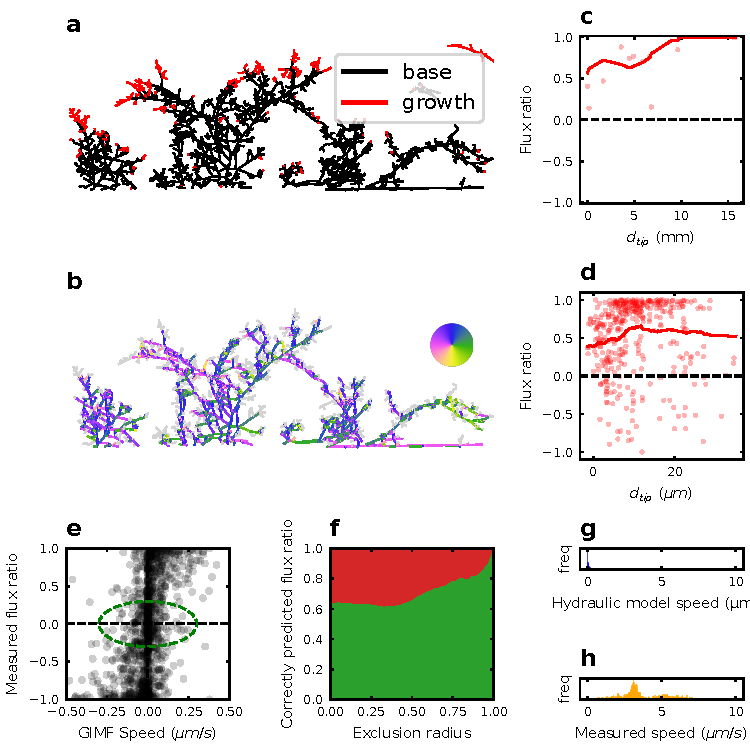
\includegraphics[width = \textwidth]{figures/figure3_lipid_flux.pdf} 
% \caption{\textbf{Demand of carbon for growth creates carbon flux at the colony scale} . \textbf{(a)} Network graph where regions that have grown between selected time-points have been highlighted in red. \textbf{(b)} Predicted motor direction through the hydraulic assumption. Color indicates direction, color wheel shows which direction. \textbf{(c)} Comparison of estimated and observed flux directions. Fluorescence is indicated in red, brightfield flux is indicated in black. Line is running average. \textbf{(d)} Aggregate flux direction in fluorescence (red) and brightfield (black) for all measured trails (number of trails = 10). \textbf{(e)} scatterplot of measured fluorescence flux ratio (y-axis) against calculated hydraulic speed (x-axis). Top left and bottom right quadrants are areas of agreement where hydraulic flux and measured flux point in same direction. Circle is example exclusion zone for \textbf{f}. \textbf{(f)} Ratio of same-sign flux ratio and hydraulic speeds. Exclusion zone removes points in \textbf{e} whose distance from the origin is less than the exclusion radius. \textbf{(g)} Histogram of absolute hydraulic speeds computed for whole network. \textbf{(h)} Histogram of all absolute fluorescence speeds measured for network.}
% \label{fig:lipid_flows}
% \end{figure}

\begin{figure}
 \centering
 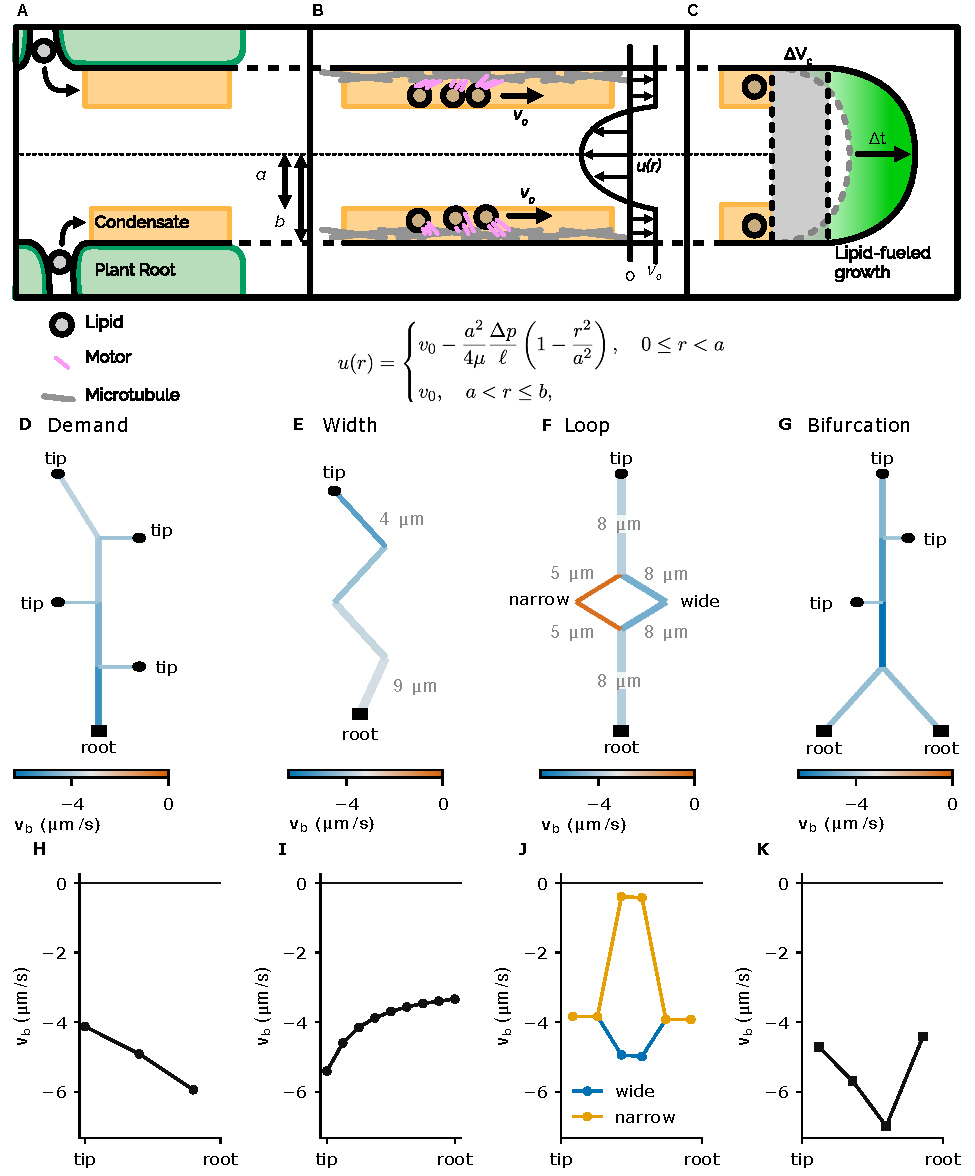
\includegraphics[width=\textwidth]{figures/Figure_4_final.pdf}
 \caption{\textbf{Proposed model of lipid flows and pressure-based backflows.} \textbf{(A)} Schematic showcase of lipid intake. Lipids are added from the plant, and go into a lipid condensate. This condensate is of radius $b - a$ where $b$ is the full hyphal radius, and $a$ is the non-condensate center radius. \textbf{(B)} Lipids in the condensate are pulled along by microtubules. This increases a pressure at the side where lipids are pulled. This increase in pressure pushes non-condensate fluids back through the center of the hyphae. \textbf{(C)} Lipids arrive at tips to facilitate growth. Some of these lipids do not aid in growth and are put back into backflow. \textbf{(D-K)} Model properties on small networks. \textbf{(D, H)} A tree-like network accumulates lipid demand going towards the root. Multiple growing tips also supply more backflow, increasing backflow velocity. \textbf{(E, I)} Width has a calming effect on backflow velocity. \textbf{(F, J)} Backflow in loops induces circularity, increasing total flow energy in the network. \textbf{(G, K)} Merges and loop additions also serve to lower the backflow velocity.}
% NOTE (5 Oct, Overleaf comments, L130): Simon: 'Lipids don't enter the network?' The condensate also consists of lipids. | Simon: Make a circuit equivalent: resistors and current drivers in parallel. | Simon: The model gives the boundary conditions; the network's resistors are also defined.
 \label{fig:schematic_model}
\end{figure}

Even our estimate of 5\% of the cytoplasm filled with lipids suggests that a significant proportion of the volume of the hyphal is filled with lipids. Such a proportion could easily lead to clogging if all of the lipids coalesce into a single phase. What then is this large fraction of neutral lipid packaged within the cytoplasm? The minimal unit of lipid packaging is generally thought to be membrane bound lipid droplets. Such lipid droplets are generally kept from coalescing by coating \cite{thiam_why_2017}. The ensemble of those lipid droplets can then form an emulsion with a set lipid volume fraction. The emulsion phase, due to the repulsive strength between the different lipid droplets, can have different rheological properties than the rest of the cytoplasm \cite{jeffrey_rheological_1976}. We assume that this emulsion is phase-separated from the bulk cytoplasm.
% NOTE (5 Oct, Overleaf comments, L134): Coco: Move to the discussion and refer to the sister paper.

We thought that this large flux of a lipid emulsion throughout the aseptate mycellium could trigger large movement of the cytoplasmic fluid in both the direction of the lipid due to viscous friction and the other direction due to the incompressibility of the fluid in the case where no water could flow out of the hyphae.
% NOTE (5 Oct, Overleaf comments, L136): Coco: This should be the beginning of the paragraph introducing Fig 4A.
This led us to propose the following conceptual model. Lipid droplets form a water-oil-like emulsion of higher viscosity that uniformly coats the internal surface of the hyphal pipe. We assume that the speed profile across the thickness of the emulsion layer was uniform at $v_0$, which could be explained by the emulsion having an effective viscosity much higher than the bulk cytoplasm. The emulsion is made up of a volumetric proportion $\theta$ of lipids and $(1-\theta)$ of water. This effectively creates an inner tube where water can freely flow. That inner pipe is smaller in radius $a$ and can allow a net flow of water $q^w_{r<a}$ to pass through it. By solving the Navier-Stokes equation in the inner pipe, setting the boundary conditions to be $v_0$ at the border of the inner pipe, one can determine the radial speed profile $u(r)$ in cylindrical symmetry to be 

% NOTE (5 Oct, Overleaf comments, L139): Coco: Update the notation to match Filipe's and link it clearly to the methods and figures (u(0), average speed, etc.).
\begin{equation}
\label{eq:speed_profile_main}
u(r) = v_0 + \frac{2(q^w_{r<a} - \pi a^2 v_0)(a^2 - r^2)}{\pi a^4}
\end{equation}
The flow of water through the inner pipe can be written as
\begin{equation}
\label{eq:net_inner_flow}
q^w_{r<a} = q^w - \pi b^2 \Theta \frac{1-\theta}{\theta} v_0,
\end{equation}
where $q^w$ is the net flow of water through the whole pipe.
Interestingly, when one assumes $q^w = 0$ as would be the case in a closed pipe system, we have:
\begin{equation}
\label{eq:max_speed}
u(0) = -v_0\left(1+2\frac{\Theta(1-\theta)}{\theta-\Theta}\right) 
\end{equation}

This result suggests a possible explanation for the bidirectional movement that we observe. For all values of $\Theta$ and $\theta$, we have $u(0)$ which is of opposite sign compared to $v_0$. It also suggests a possible explanation for the spatial and temporal variation of speeds. The spatial variation of $\Theta$ (Fig. \ref{fig:carbonflow}f) indeed directly contributes to the magnitude of the backflow speed.
 
A direct consequence of such a conceptual model is that a single pipe insulated at both ends where the movement of lipid is maintained will still exhibit bidirectional flows (Fig. \ref{fig:schematic_model}B). We therefore isolated a segment of $\sim$1mm of hypha from the rest of the network by physically cutting the neighboring edges. Preliminary experiments had shown that severing the hyphae in this way leads to a temporary spilling of the cytoplasm that quickly stopped because of some physical clotting. A similar clotting phenomenon after hyphal injury was recently reported in another (non-mycorrhizal) fungal species that involves a shear sensitive protein called gellin \cite{nguyen_fungal_2021}. We then observed fluid movement inside the isolated edge at high resolution (Fig. \ref{fig:fig5_plug}B, \href{https://www.dropbox.com/scl/fi/ors0lqpopi5yymh6e79o9/SIvideo3.avi?rlkey=lfbndih3j9fg033892r7t8cw5&dl=0}{SI video 3}). We found that fluid was still moving and that flow was still bidirectional (Fig. \ref{fig:perturbations}D, E). Flow speed was of similar magnitude (3$\mu$m/s) in both directions. This observation provides further evidence against the idea that a significant proportion of fluid movement could be explained by growth induced mass flow. We indeed observed a fluid movement of similar magnitude as in the full network while our isolated segment did not show any growth. Our model is instead fully compatible with the maintenance of bidirectional fluid movement in the disconnected hypha. According to our model, after cutting, the active entrainment of the lipid suspension phase could be maintained at its fixed speed (3$\mu$m/s). Because the isolated hypha is clotted at both ends, it is reasonable to assume that the net water flow through the whole pipe is zero. Furthermore, with the additional assumption that the volume fraction of the lipid suspension is negligible, we directly obtain from equation \ref{eq:max_speed} that the speed in the opposite direction should also be maintained and should be close to $v_0$. Analysis of the kymograph revealed that the speed in both directions is indeed close to $3\mu m/s$.
% NOTE (7 Oct, section cut, recomputed with transport_paper figure3/d_e_segment_cut_results.py = Fig 3D/E): 4 positions, post-cut videos 0.07-1.8 h after the cut (median 0.3 h). Medians pre -> post, um/s: bright-field to tip 2.98 -> 2.60, to root 3.62 -> 3.15; Nile Red to tip 2.82 -> 2.52, to root 3.16 -> 1.96. So '~3 um/s in both directions' holds in bright-field. L93 ('tip direction almost unaffected, root direction more affected') holds in Nile Red (-11 % vs -38 %), but in bright-field both drop ~13 %. Also: 'Fig. fig5_plug B' for the isolated-edge video points to the percentile panel of the current Fig 5.

Our conceptual model seemed to be well validated by the data at the individual pipe level. However, we wanted to know what its consequences would be at the network level. Could it explain the observed variation of speed in space and time? When establishing the speed profile through the pipe, we were also able to derive the pressure gradient along the idealised hyphal pipe. For a pipe of length $L$ the expression for the pressure drop was analogous to an electrical voltage drop where a voltage generator and a resistor would be put in parallel (Methods). Because fluid movement happens at low Reynolds numbers in our system and the entrance length in each individual hyphal pipe is close to its diameter, the approximation of an infinite length cylinder we used to derive flow profile in a single pipe is still justified in the network context. A network of connected pipes is then analogous to a network of these individual circuit elements.
% NOTE (7 Oct, entrance length): holds. At Re << 1 the entrance length is ~0.6 D; with v ~5 um/s, D ~5 um and water viscosity Re ~2.5e-5.

Such an electrical circuit equivalent of the network can be solved with linear algebra using Kirchhoff's law at each intersection, and requiring that the sum of pressure drops around loops in the network be zero (Methods). As in the case of growth induced mass flow discussed above in \nameref{subsec:lipid_flow}, we set the sink magnitude at each node to correspond to newly created volume $\Delta V_k$ and added a global source node. A number of properties can be shown in toy networks (Figure \ref{fig:schematic_model} D-G). Tree networks aggregate backflow into their central trunk,   increasing flow rate (Figure \ref{fig:schematic_model} H). This increase in flow rate can increase backflow speeds, if not modulated by a greater flow capacity, which can be done by increasing the diameter (Figure \ref{fig:schematic_model}E, I). One feature this model also predicts is circularity in added loops, specifically if these have a width imbalance. The pressure difference that has to be serviced by both makes the wide arm flow faster, and the narrow arm far slower than in just a single edge. While this increases energy overall in the network, these induced circularities likely facilitate the distribution of nutrients in the backflow throughout the network (Figure \ref{fig:schematic_model}F, J). Finally, anastomoses can reduce the load on a tree-like network by routing backflow through multiple edges. This way, pressure differences in tree-like sections get reduced, and backflow nutrients can be accessed by more parts of the network.
% NOTE (7 Oct, terminology): 'width imbalance', 'wide arm', 'narrow arm' here, and 'Width has a calming effect' in the Fig 4 caption (E, I): diameter wording per the width rule.

This allowed us to predict on each edge what the net volumetric rate of fluid movement $q^w$ would be and then the direction and magnitude of the flow speed in the inner tube of each edge of the network (Fig \ref{fig:fig5_plug}). We found that our model captures salient features of the bidirectionality of flow observed across all edges. The speed was higher in those central hyphae where the lipid density was also higher, which was explained by the larger proportion of the volume of the pipe occupied by the lipid suspension moving in $v_0$ and dragging water with it (\ref{eq:max_speed}). In tree-like parts of the network, the net volumetric flow of water through the whole pipe $q^w$ is close to zero because the amplitude of growth induced mass flow is negligible (Fig. \ref{fig:carbonflow}d,e). Then, the movement of water in and around the suspension of lipid droplets can only be compensated for by faster speeds in the opposite direction in the inner pipe.
% NOTE (7 Oct, SI references): Fig. carbonflow f (L174) and d,e (here) are among the wrong SI files (FigS2-S5, transport_paper#129); no figure behind these claims until replaced.

\subsection*{Lipid generated backflow}
% \begin{figure}
% \centering
% 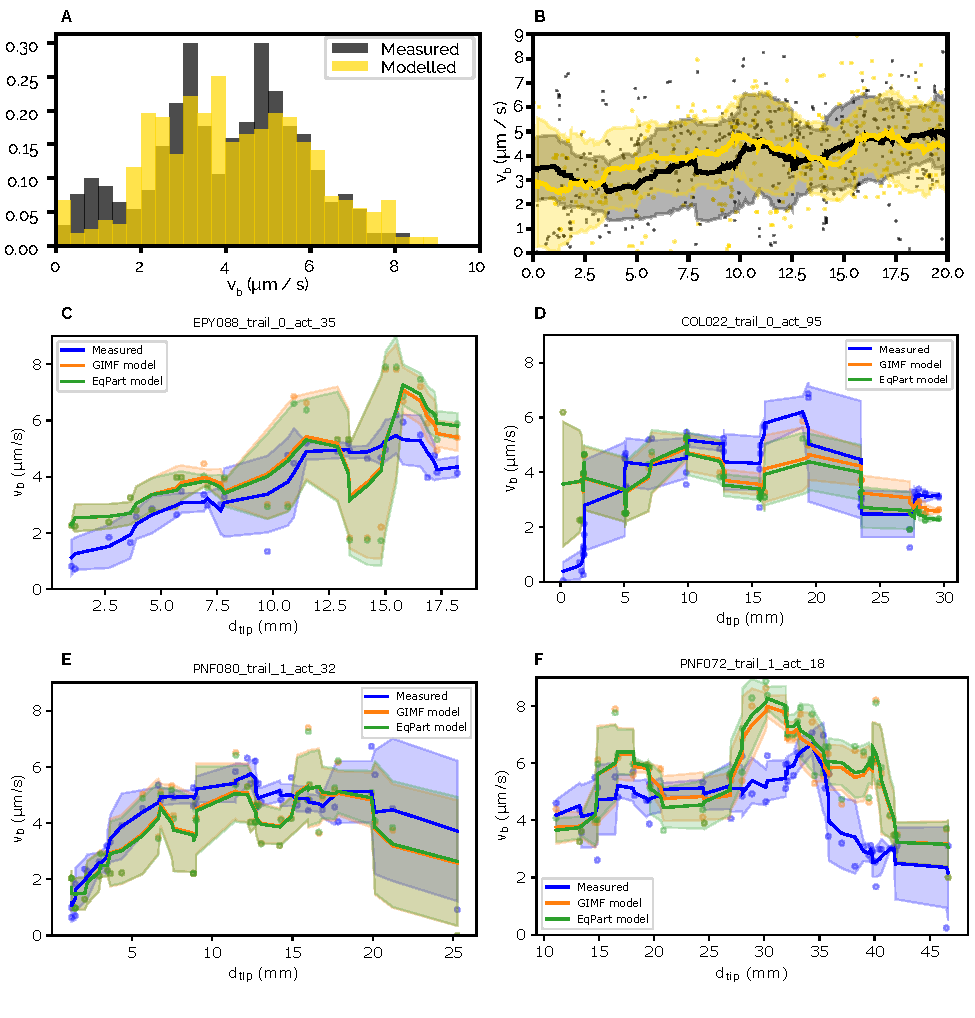
\includegraphics[width=\linewidth]{figures/Figure_5_final.pdf} 
% \caption{\textbf{Lipid movement induced backflow.} \textbf{(a)} 
% Results on modelling backflows. \textbf{(A)} Histogram comparison between measured and modeled backflow speeds. \textbf{(B)} Scatterplot and rolling means of measured and modeled speeds against tip distance. Rolling mean and standard deviation are also shown. \textbf{(CDEF)} Comparisons across 4 plates of measured backflow speeds and modeled backflow speeds.}
% NOTE (5 Oct, Overleaf comments, L170): Simon: Make it more varied and pointed: needs an example of falloff in a highly loopy region, and one of accurate predictions over time. | Simon: Minus sign in front of v_b? Add individual hyphae and the hypha-highlighted network; show panel B the same way as panel 1F. | Simon: 'Quantified agreement?'
%  \label{fig:backflows}
% \end{figure}

\begin{figure}
    \centering
    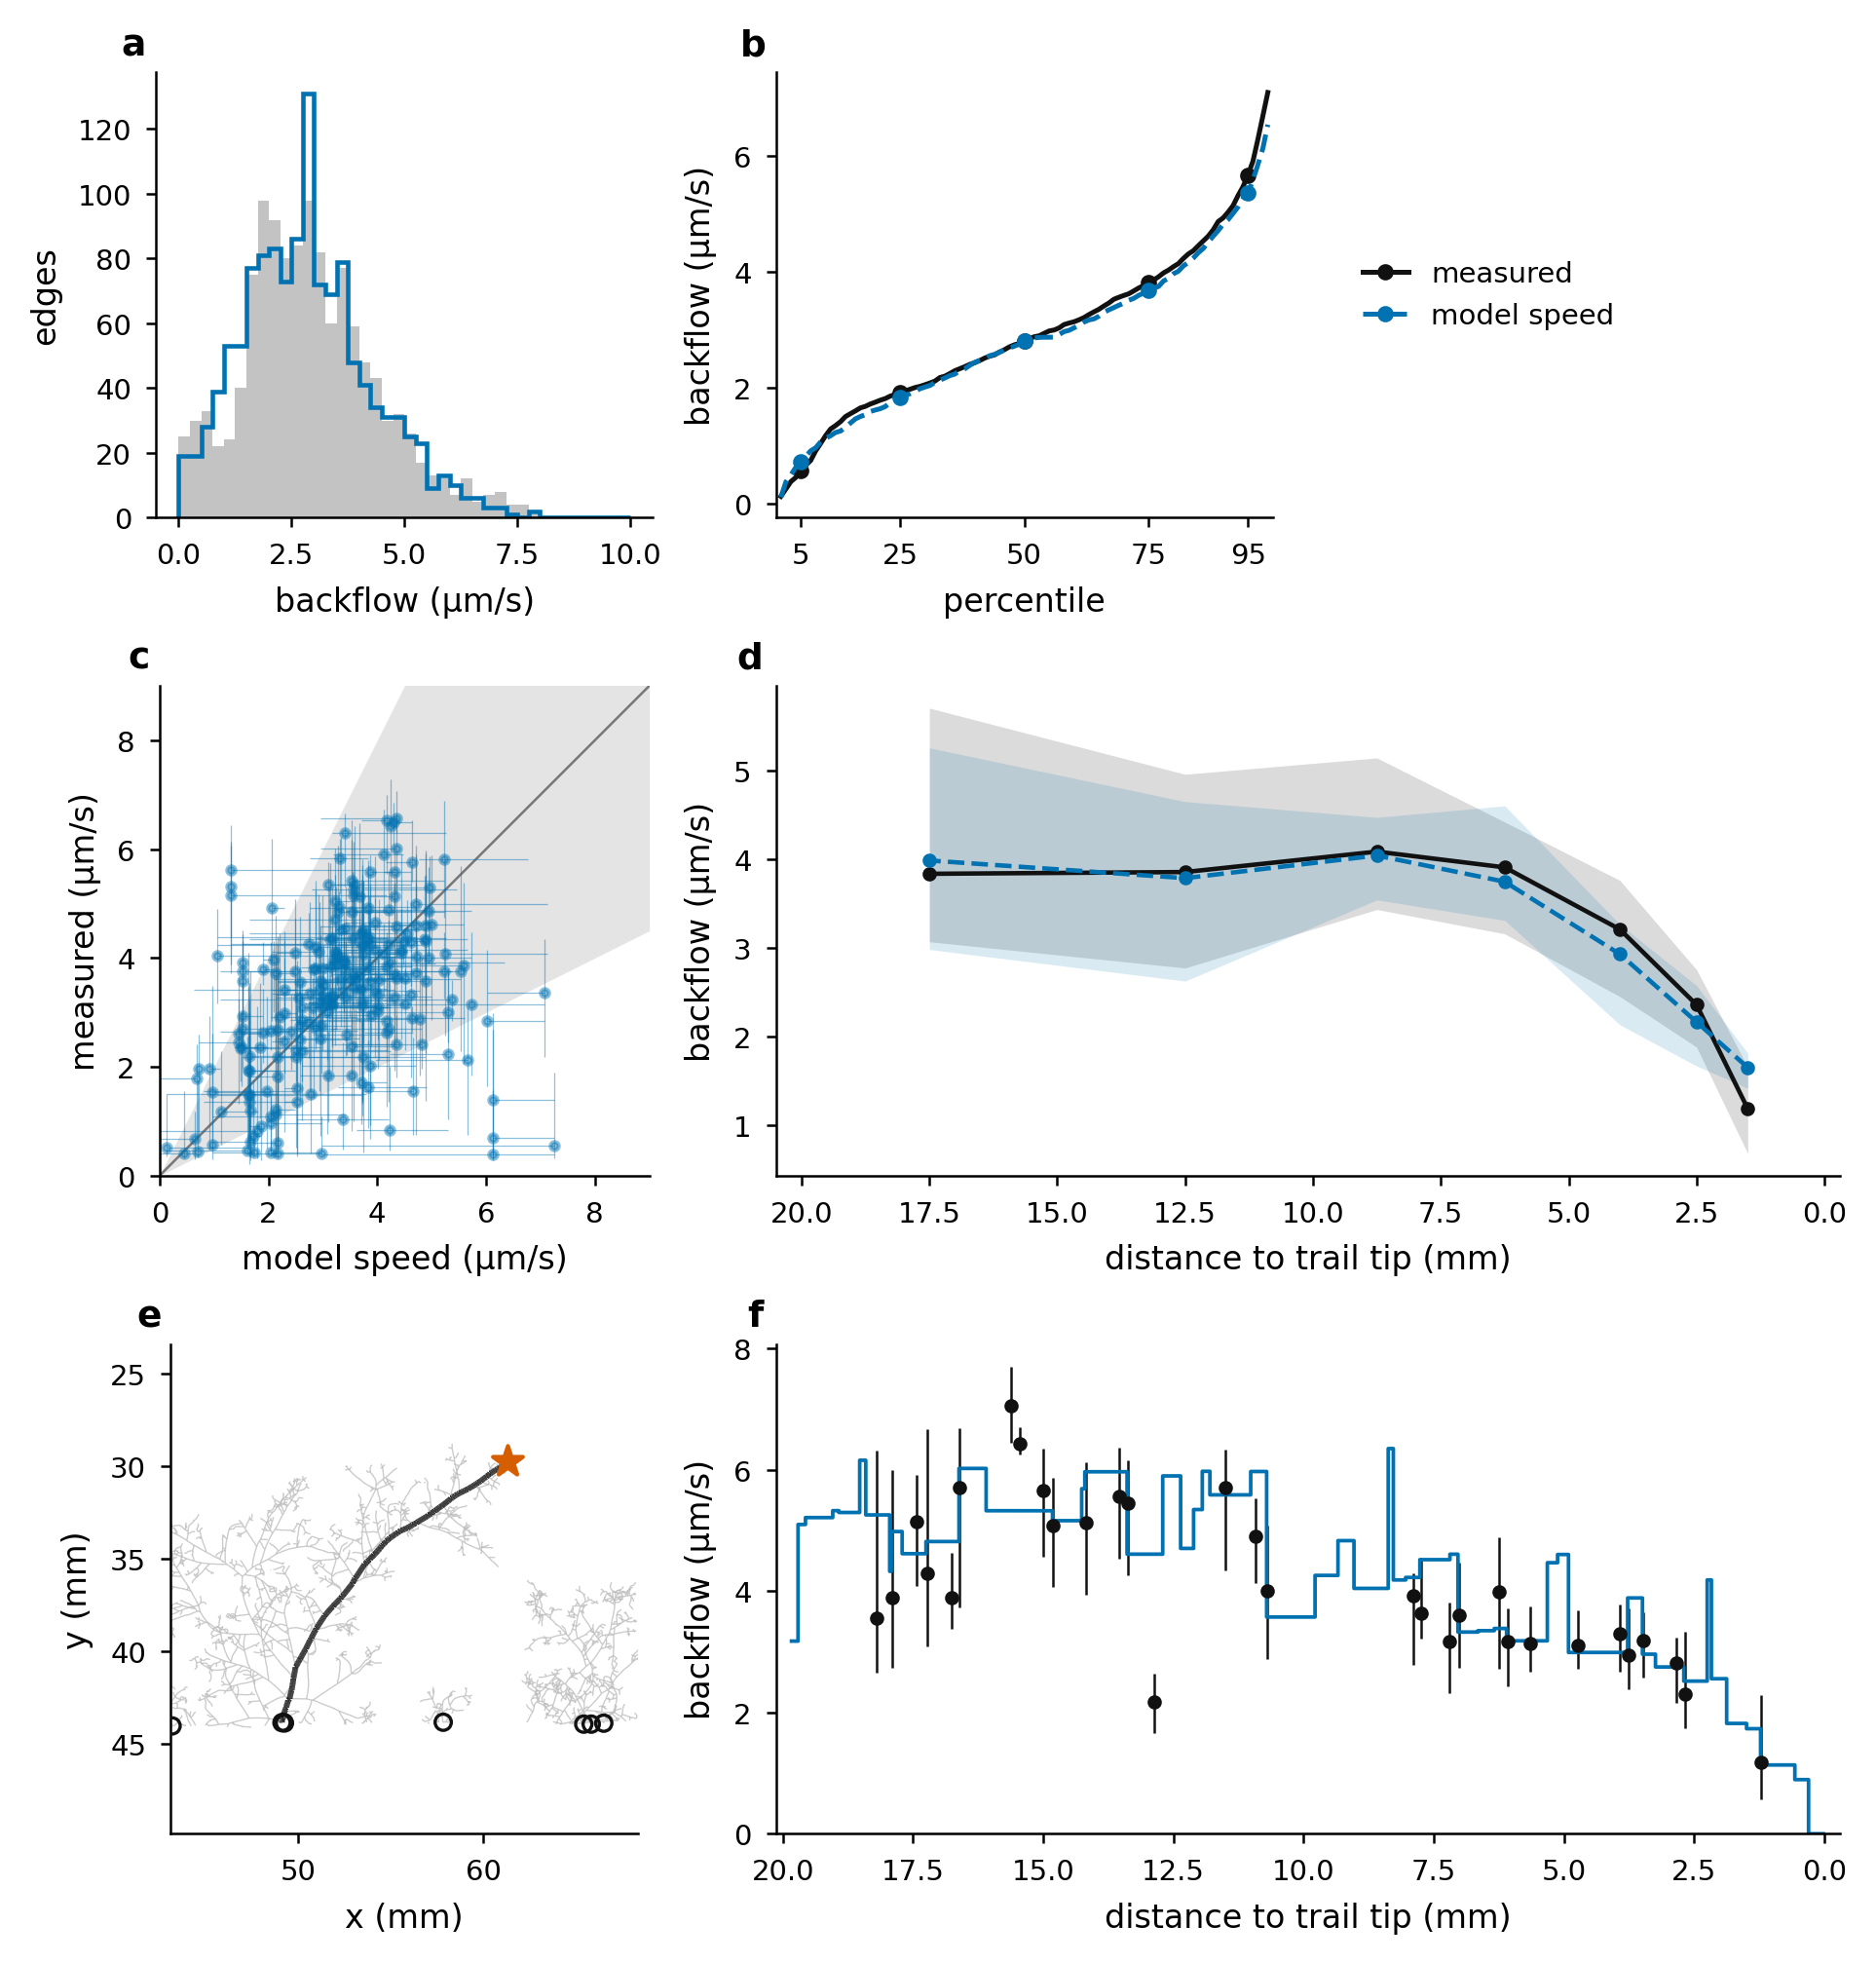
\includegraphics[width=\linewidth]{figures/fig_plug_model.png}
    \caption{
Measured brightfield backflow speed against the model-predicted speed (blue). \textbf{(a)} Distribution over every measured edge with model output (1,248 edges in 11 sessions). \textbf{(b)} Percentiles of the same distributions from the 1st to the 99th. \textbf{(c)} Measured against predicted on the 232 trail segments within 10 mm of the trail tip. 84\% of points fall within a factor of two of the measured speeds. Vertical error bars: 25th–75th percentile of the measured velocity pixels of the videos covering the segment; horizontal error bars: range of the prediction over the trail's segments within $\pm0.5$ mm; grey wedge: within 2x; line: identity. \textbf{(d)} Backflow on trail segments against distance to the trail's tip at the session, in bins of 0–1, 1–2, 2–3, 3–5, 5–7.5, 7.5–10, 10–15 and 15–20 mm holding 4, 16, 23, 56, 63, 70, 95, 89 measured segments; line: bin median, band: 25th–75th percentile (grey for measured, blue for the model speed). \textbf{(e)} The session network of EPY2412A088 t55 with trail (black), its tip at the session (star) and the annotated roots (circles), in image coordinates. \textbf{(f)} Backflow along trail in e (31 measured segments, bar: 25th–75th percentile) with the prediction, within 2x on 97 \% of segments with median.}
    \label{fig:fig5_plug}
\end{figure}
% NOTE (7 Oct, Fig 5 caption numbers): fig_plug_model.png was committed 30 Sep as '1,566 edges in 15 sessions'; the caption says 1,248 edges in 11 sessions. After the 3 Oct no-cut rebuild (transport_paper manuscript/figs4-6_rebuild_2026-10-03.md) the physical-input global solve gives 1,590 edges, fold error x1.45, 77 % within 2x, and 79 % of trail segments within 2x (caption: 84 %). The bin counts and the 97 % in (f) were not re-derived.

Could our conceptual model at the network level quantitatively explain the variation of speeds observed throughout the networks (Fig.\ref{fig:hyphal_profiling}f)? To answer that question, we first plotted the distribution of observed and modeled flow speeds for all edges observed in high magnification (Fig.\ref{fig:fig5_plug} A). We found that the model could overall explain well the distribution of speeds from 1.5 to 6 $\mu m/s$. Speeds slower than $v_0$ were explained by the existence of loops in the network that led to a net circulation of water through some of the pipes that crossed the same direction as lipid flux. According to equations \ref{eq:net_inner_flow} and \ref{eq:speed_profile_main}, when $q^w$ is large enough and positive, $q^w_{r<a}$ can also be positive and larger than $\pi a^2 v_0$, which can lead to the absolute speed being lower than $v_0$. During the length of a hypha, our model could explain the gradual increase of flow speed when moving away from the tip, as well as the sudden decrease which seemed to coincide with entering regions with multiple alternative paths due to anastomoses to the root (Fig.\ref{fig:fig5_plug}F). Our model could also explain the increase in flow speed over time at specific locations (Fig.\ref{fig:fig5_plug}e). 
% NOTE (5 Oct, Overleaf comments, L182): Simon: Need a concrete example of this. | Simon: 'Also good to-do for fig 5.'
% NOTE (7 Oct): '1.5 to 6 um/s' fits the rebuild (global solve 5-95 %: 1.5-6.6 vs measured 1.5-6.8 um/s). 'Slower than v0 explained by loops' does not fit it: 53 % of the global solve's misses are too slow. '(Fig. fig5_plug e)' for the increase over time: panel e is the network map, no time series. '(Fig. hyphal_profiling f)' is lowercase where the other panel letters are now capitals.

Our simple physical model can therefore explain a wide variety of our experimental observations. At the single hypha level, it provides an explanation for bidirectional fluid flow. At the growing network level, it is compatible with the observed non-trivial spatio-temporal variations in flow speeds. Such a physical explanation of bidirectional transport in AM fungal networks has direct consequences on symbiotic trade. Because the movement of lipids generates fluid flow in the reverse direction, the proportionality of resource exchange could emerge directly from this physical coupling. 

 % We wanted to know whether the lipid movement induced backflow could explain the proportionality of resource exchange. We assumed that the concentration of phosphorus in the water of the inner tube was constant and that the input carbon flux varied. We found that, under this assumption, the carbon flux from the plant and the phosphorous flux from the fungal colony were maintained proportionally (Fig. \ref{fig:hydraulic_proportionality}b). To obtain a proportionality factor of $1/3$ $\mu g$P / $\mu g$C, as previously found (see Chapter \ref{chapt2}), we had to set the concentration of P to $\approx 1.9 mol/L$ which is much higher than the concentration typical found in plant cells of 5-20$mmol/L$ \cite{bieleski_phosphate_1973}.

\section*{Discussion}
Our results suggest that the lipids preferentially move in a direction informed by fungal growth. They also strongly support the idea that this movement of lipids could be actively driven by molecular motors moving in one direction on polar cytoskeletal filaments. This network of filaments inside the fungal network is mathematically equivalent to a weighted oriented graph, where the weight of a given edge can represent the number of cytoskeletal filaments, allowing molecular motor movement. It is unclear how this oriented network organizes to maintain a coherent intensity and polarity with growth. 
% NOTE (8 Oct, context in other organisms; guest_multiple_2026 now in PhD.bib, Curr Biol 36, full text read): Filoreta ramosa, a reticulate (branching and anastomosing) amoeba. Actin protrusions explore, microtubule uptake stabilises branches. Nuclei, lysosomes and mitochondria move both ways at 5.3, 7.3 and 8.3 um/s on microtubules; speed rises loosely with branch diameter (R2 0.54, 1.5-6.5 um; wider branches hold more MTs) and slows at nodes. Nocodazole: max nuclear speed -27 %, run length -33 %; dynein inhibitor ciliobrevin D: speed -70 %, remaining nuclei still bidirectional; latrunculin < 25 %. MT nucleation (gamma-tubulin, GCP3) sits at branch nodes, not at nuclei. They contrast Physarum (pressure-driven streaming) with Filoreta (motors) as two network solutions; AMF here would use both, one per direction. Caveats: amoeba, no wall or turgor, single organelles not a lipid stream. To-tip speed vs diameter in our data requested from the 'Fluorescence slow bias?' session (8 Oct).
% NOTE (8 Oct): our data show the same trend as Filoreta: to-tip speed ~ D^0.5 (see the note at the summary paragraph); to-root rises faster in bright-field (slope 1.09 [0.97, 1.20]; to-root/to-tip ratio slope 0.62), not clearly in Nile Red (ratio slope 0.16 [-0.05, 0.37]). The model's constant motor speed v0 is being tested against v0(D) in transport_paper#134.

Each edge of the network has a growth inherited orientation that is associated with the polarity of tip extension. It is likely that part of the network of transport filaments simply orients in the direction of tip growth at the moment of its creation and persists in that direction over longer timescales.

One way of thinking about the system is that it is mainly driven by supply. Although in this paper our approach was to estimate what the flux of carbon was in each edge of the network from growth observation, it is possible that from the fungal point of view things work the other way around. Growth would mainly emerge from the network's underlying molecular motor track organization.

This has the advantage of solving an informational bottleneck. If a tip grows at one end of the network, how is the information about its carbon demand transmitted to the root-fungal interface where that carbon will eventually come from? Instead of needing information transmission to match supply and demand and orient carbon fluxes accordingly, fungal tips could grow and branch according to the carbon supply of the existing network of molecular motor tracks. Indeed, the net flux of lipid across the colony could be entirely determined by its orientation (track direction) and intensity (number of parallel tracks assuming tracks are saturated with motors) as well as by the plant supply (source). The growth might then simply occur at a rate limited by the network-determined supply of lipids.

However, some abrupt topological changes, such as anastomosis or the colony abandoning growth in a specific region of space, could require a reorganization of the cytoskelal filaments. It is unclear how that reorganization is modulated in a way that allows one to maintain a flux of carbon that is consistent with the general fungal growth strategy. Depending on the timing of the reorganization, it is also likely that the flux of lipids moving on microtubules will not always follow the Kirchhoff law at some intersection. Because lipids are incompressible and cannot accumulate in a node, this means that they will be recirculated in the internal cytoplasmic flow. This phenomenon could explain the observation that lipids can also move in two directions in fungal hyphae.
% NOTE (8 Oct): Guest & Dawson 2026 (guest_multiple_2026) infer antiparallel MT arrays where branches growing from opposite directions fused (nocodazole: such branches retract toward both nodes at once): another lineage in which anastomosis leaves tracks pointing both ways in one edge. In our model the motor direction comes from the hydraulic solve or from the growth direction (both open, Simon 8 Oct); no evidence of motor switching yet.

We see that bidirectional resource movement and trade could be largely mechanically mediated. Such a control mechanism has the advantage of being robust because the proportionality of flow is embedded in the physical properties of the system and, therefore, does not require additional biological control. However, in our model, the path taken by the phosphorus in the network is strongly dependent on its relative cumulative hydraulic resistance and, therefore, on the edge radii. Radial adaptation could constitute a flow control mechanism. However, we never observed hyphal external radii diminishing. Full control would probably require an additional ingredient of radial shrinkage. 
% NOTE (9 Oct, C/P framing, Simon: frame on motor-carried carbon; transport_paper#128, analysis feat/cp-production fb436c6): in the global solve the volume returning into the roots equals the motor stream leaving them in all 15 sessions, so P out (constant [P]) is proportional to motor-carried carbon (theta x motor stream) by construction (log-log slope 1.000). This is a property of the mechanism, not a fitted result. Against growth carbon it does not hold: slope 0.19 (95 % CI -0.47 to 0.86, R2 0.03) over 15 sessions; on STR2307A112 growth carbon rises 4.7x over 5 sessions while the return stays flat (0.0050-0.0066 uL/h).
% NOTE (9 Oct, needed P concentration): with P:C = 1/3 to 1/4 ug P per ug C, motor-carried carbon at theta 0.05 needs [P] = 0.38 to 0.29 mol/L in the returning fluid, proportional to theta (0.19 mol/L at theta 0.025, 0.76 at 0.10); plant cells 5-20 mmol/L (bieleski_phosphate_1973, range not re-checked). Reaching 20 mmol/L needs theta ~0.0026, at which the motors carry ~0.19x the carbon growth uses (3.7x at theta 0.05, median); so a plausible [P] and feeding growth pull theta in opposite directions. The old analysis (commented-out paragraph at the end of the Results) needed ~1.9 mol/L.
% NOTE (9 Oct, Bisot et al. 2026, full text checked, PMC12891005; bisot_carbon-phosphorous_2025): exchange rate kappa = Phi_C / Phi_P by MASS, ~3-4 ug C per ug P ('3 to 4 C/P'; Fig. 5 fronts at kappa0 = 3 and 4), set by host genotype, not by fungal strain or P availability. Their carbon is EXPENDED carbon (CUE 50 %, i.e. twice the carbon built into biomass, spores included), a growth-based quantity, not the motor-carried carbon of this framing. Also: >= 85 % of absorbed P reaches the root within ~100 h (P absorbed ~30 % of fungal dry mass if none were transferred, vs <= 4-5 % P measured in hyphae).

In our model, we assumed that water could not flow out of the hyphae except at the hyphal-root interface. However, it is likely that the ERM hyphae are covered with aquaporins that let water in and out. In that case any kind of water potential gradient between the inside and outside of the hyphae could produce influx or outflux of water at any point of the network. The resulting system would be analogous to the xylem-phloem system of plants. In that case, the sugar loaded phloem generates an influx of water from the xylem. This in turn generates a net flux of water through the phloem. Any kind of osmolyte that would be produced inside the fungal network could very well drive a similar osmotic pump by changing the overall flow distribution in the network. Although we cannot exclude such effects from playing a role in the transport of resources within the AM colony, it is not incompatible with the mechanism of bidirectional flow described in this paper. Regardless of the contribution of other mechanisms, our results strongly suggest that lipid movement results in some fluid flow in the opposite direction. And such backflows must be playing a significant role in the full picture of AM fungal flows. The framework developed here can also be flexibly expanded to include the effect of other kinds of carbon demand, such as spore growth or hyphal maintenance. By adding current generators at different places in the network to represent the influx or outflow of water due to water potential mediated flow of water through aquaporin, it is also possible to account for additional transport mechanisms.
% NOTE (5 Oct, Overleaf comments, L201): Simon: 'Maybe even not': AMF lacks genes associated with passive water-exchange hydroporins.
% NOTE (7 Oct, aquaporins): R. irregularis (then G. intraradices) has two functional aquaporins, GintAQPF1 and GintAQPF2 (Li et al. 2013, New Phytol 197:617-630, doi:10.1111/nph.12011): expressed in yeast they speed the volume response to osmotic shock. Found by web search, full text not read; not in PhD.bib.
% NOTE (7 Oct): now in PhD.bib as li_first_2013.

\section*{Bibliography}
\bibliographystyle{bxv_abbrvnat}
\bibliography{PhD.bib}

%  CONFIGURE SUPPLEMENTARY FORMAT

\onecolumn % go back to one column
\fancyhead{} % make sure we get no headers
\renewcommand{\floatpagefraction}{0.1}
\lfoot[\bSupInf]{\dAuthor}
\rfoot[\dAuthor]{\cSupInf}
\newpage

\captionsetup*{format=largeformat} % make figure legend slightly larger than in the paper
\setcounter{figure}{0} % reset figure counter for Supplementary Figures
\makeatletter
\renewcommand{\thefigure}{S\@arabic\c@figure} % figures numbered S1, S2, ...
\makeatother

%  MAIN TEXT

\newpage
\section*{Supplementary Information}

% -----------------------------------------------------------------------
% FIGURE S1
% Actively referenced in main text (line 48):
%   "method, SI Fig. \ref{fig:speed_flux_extraction_real_data}"
% Content: pipeline for extracting directional (tip-ward / root-ward)
%          speeds from bright-field kymographs.
% -----------------------------------------------------------------------
\begin{figure}[hbt!]
\centering
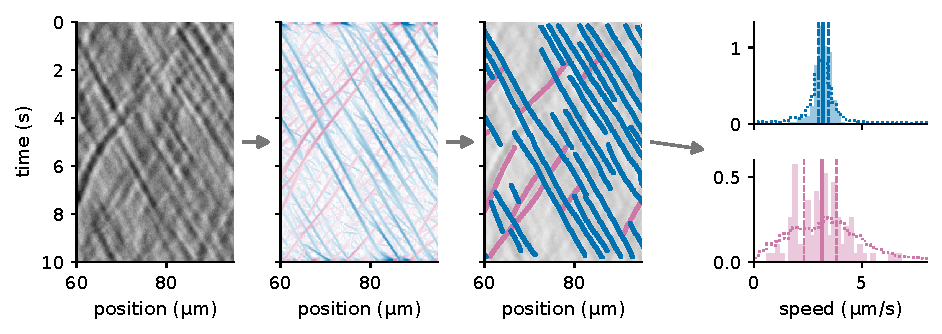
\includegraphics[width=\textwidth]{suppfig/FigS_streak_pipeline.pdf}
\caption{\textbf{Method for extracting directional speeds from kymographs.}
\textbf{(A)} TODO.
\textbf{(B)} TODO.
}
\label{fig:speed_flux_extraction_real_data}
\end{figure}

\clearpage

% -----------------------------------------------------------------------
% FIGURE: positions of all flow videos
% Actively referenced in main text (Results, "about 1500 flow videos"):
%   "SI Fig.~\ref{fig:video_positions}"
% Content: every filmed session's network with all video positions.
% Generated by transport_paper Working_notebooks/manuscript_figures/figS_video_positions.py
% -----------------------------------------------------------------------
\begin{figure}[hbt!]
\centering
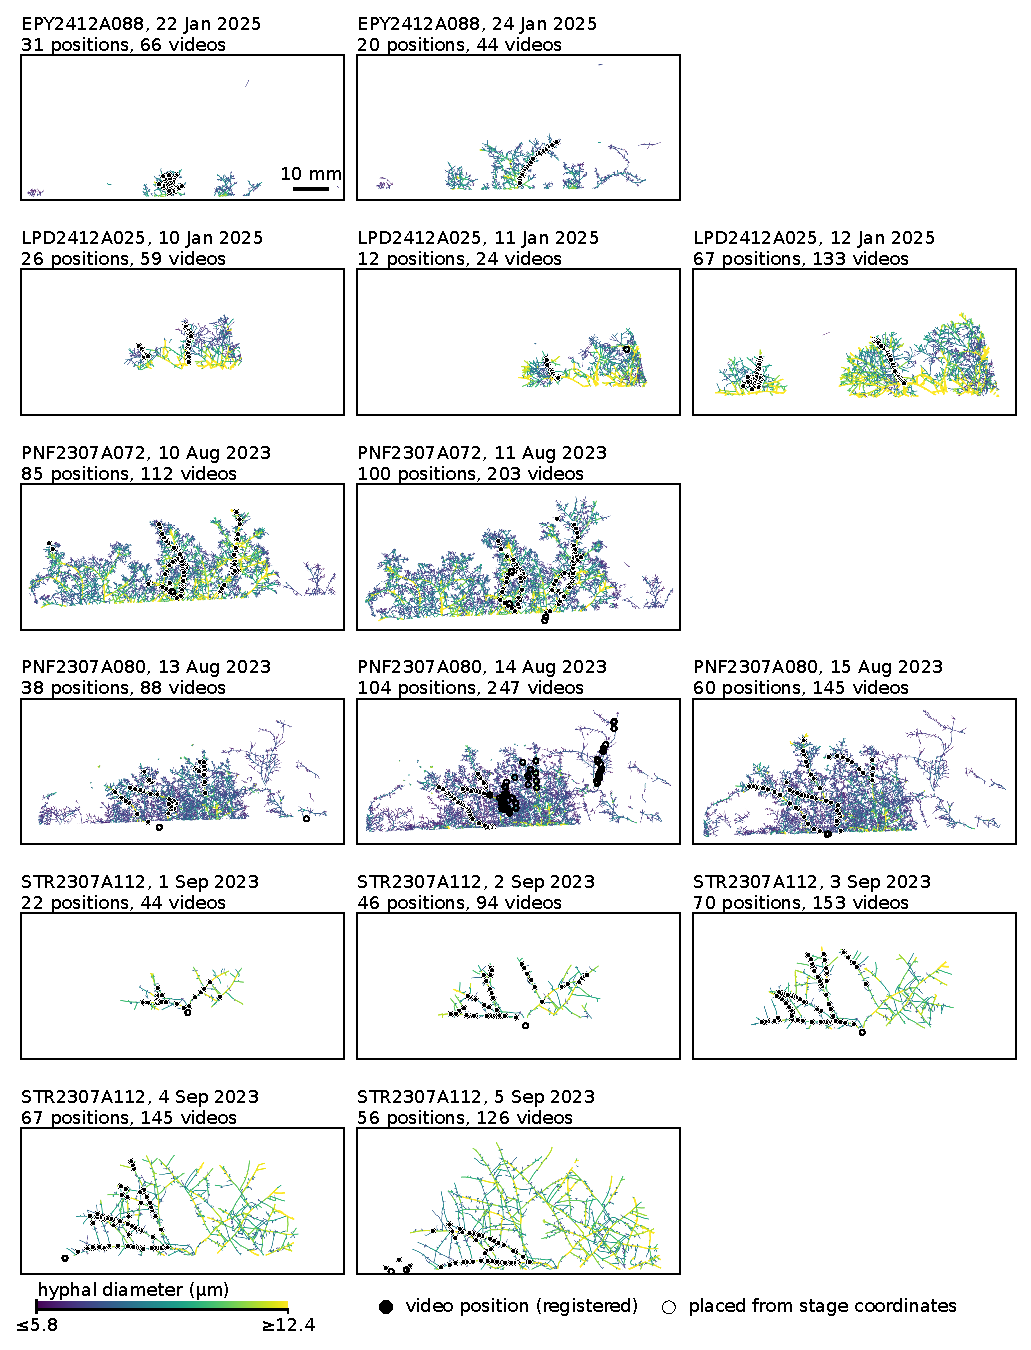
\includegraphics[width=\textwidth,height=0.85\textheight,keepaspectratio]{suppfig/FigS_video_positions.pdf}
\caption{\textbf{Positions of all flow videos.}
Each panel shows the network of one filmed session (5 colonies, 15 sessions, in time order per colony), drawn as in Fig.~\ref{fig:hyphal_profiling}A,B: colour indicates hyphal diameter.
Dots mark the 804 stage positions at which the 1,683 videos were taken (a bright-field video, mostly followed by a Nile Red video at the same position).
Filled dots are placed at the hyphae their videos were registered to; open dots (74 positions without a registered video) are placed from the microscope stage coordinates.
The LPD2412A025 sessions (10--12 Jan 2025) are days 10--12 of Fig.~\ref{fig:hyphal_profiling}B. All panels share the 10~mm scale bar.}
\label{fig:video_positions}
\end{figure}

\namedsubsection{Lid-on and lid-off flow videos}{subsec:si_lid}
% NOTE (10 Oct): section text to be written by Simon; cited from the main text (peristaltic streaming, flow reversals). Facts from transport_paper#121 (Simon, 2 Oct: a stated condition of the flow videos, Methods supplement):
% NOTE (1): sessions filmed with the lid off, before late 2023, show back-and-forth flow driven by air flow over the plate (docs log 2026-10-01-a-lid-off-dropbox-4x-session-showed-the-motion-gate-passing-drifting-static-texture.md).
% NOTE (2): the paper's sessions were filmed with the lid on; still to confirm for all sessions (Methods \todo at the flow-video paragraph).
% NOTE (3, open before writing): which sessions/plates were lid off and whether any enter the paper's tables; Snellius jobs 27439881 and 27439919 (2023 lid-off videos: curvature, synchronous swings, resolution) not yet read.

\namedsubsection{Size of the isolated segment}{subsec:si_segment_size}
% NOTE (10 Oct): section text to be written by Simon; cited from the main text (section cuts, "does not require the long range connectivity"). Facts from docs log 2026-09-29-registering-the-cut-videos-shows-the-stage-coordinates-are-off-by-millimetres-and-the-smallest-isolated-piece-loses-the-most-flow.md; analysis transport_paper Working_notebooks/figure3/section_cut_registered.py (branch feat/section-cut-registered 4a34453), outputs fig_outputs/perturbations/section_cut_registered/videos.csv.
% NOTE (1, data): cut-day videos registered by hand (Simon) onto arc-unit STG stores anchored on the last frame before the cut: LPD2412A025_t77, EPY2412A104_t82, EPY2412A084_t73, LPD2412A009_t90. LPD2412A023 cannot be registered (its segmented frames miss the long hyphae around the cut site).
% NOTE (2, piece size from the network): a piece is isolated when the cut splits it off its component (cut mark severs every edge within max(50 um, 2.5 map px)). Stores have segmentation gaps, so the 24 and 73 mm pieces may still be joined in reality.
% NOTE (3, post/pre speed on the same STG edges, 0-30 min / later): EPY2412A104, inside a 4.6 mm piece between two cuts (hand value 4.3 mm): 0.74 / 0.18 at 35-68 min; LPD2412A025, 24 mm piece, 1.4 mm from the cut: 0.26 / 0.68 at 80-326 min; EPY2412A084, 73 mm piece, 3 mm away: 0.78 / 0.84 at 30-58 min; LPD2412A009, still connected, 1.9 mm along the network: 0.80 / 0.66 at 93-119 min; at a cut stub (EPY104, LPD009): 0.10-0.50 / ~0.10.
% NOTE (4, reading in the log): the smallest isolated piece loses the most flow over time; whether the size dependence holds needs more than one small piece. Flow did not stop in any piece (main text), but at cut stubs it fell to ~0.1 of the pre-cut speed.
% NOTE (5, caveats): stage coordinates are unreliable on every cut plate (positions off by 0.2-2.3 mm; videos placed by frame matching and Coco's map labels instead); registrations give the edge, not the position along it; EPY104 videos 22 and 28 may sit outside the piece (Coco's labels vs registration). The writeup science/section_cut_sites.typ (rhizosphere PR #240) still carries the older stage-position numbers.

\namedsubsection{Selection bias of the filmed hyphae}{subsec:si_video_selection}
% NOTE (10 Oct): section text to be written by Simon; the facts (definition, numbers, caveats) are in the note above the figure below.
% NOTE (10 Oct, outline for this section, facts only; sources: transport_paper feat/bc-selection-bias d2054b7, manuscript/bc_selection_bias.md, #130):
% NOTE (1, why): the flow videos were taken by eye on runner hyphae where the two streams could be told apart (main text, Results opening). Speed statistics therefore describe the filmed hyphae, not the network as a whole; this section measures how different the filmed edges are, so the reader can judge how far the results generalise.
% NOTE (2, measure): betweenness centrality (BC) as defined by Oyarte Galvez et al. 2025 (oyarte_galvez_travelling-wave_2025, after freeman_set_1977): for each edge, the number of shortest paths (by edge length; equal-length paths share 1/sigma each) from every node of the session network to the root compartment, i.e. one super-node joined at zero length to all annotated roots; divided by the number of source nodes, so it is the share of nodes whose route to the root crosses the edge. Edges with BC = 0 are left out (62,469 of 1,139,071; 42 filmed). Variant: sources = growing tips only.
% NOTE (3, groups): filmed edges = store edges that carry a video mapping (1,972 with BC > 0, 15 sessions on 5 plates). References: all edges of the same session networks (1,076,602), and, to separate selection from where the plates were filmed, the edges inside the convex hull of the filmed positions (310,967).
% NOTE (4, result): filmed edges sit at a median 82nd percentile of BC within their own network (IQR 54-95); every session's median is above 50 (73-96; Wilcoxon over sessions p = 6e-5). Median log10 BC: filmed -2.40, all -3.80, inside the hull -3.83, so the shift is selection, not spatial extent. Per session, P(filmed > other edges) 0.63-0.89. Tips-only BC gives the same picture: 80th percentile (IQR 61-92), session medians 64-95; rank correlation of the two BC variants across edges 0.78.
% NOTE (5, what else differs): filmed edges are thicker (store diameter 10.0 vs 7.8 um), slightly closer to a growing tip (4.3 vs 4.8 mm), and far less often tree-like (15 % vs 36 %; 33 % inside the hull). BC and diameter covary, so the diameter difference is not a separate selection.
% NOTE (6, consequence for the speeds, panel C): among filmed edges, bright-field median speed rises weakly with log BC in both directions: Spearman 0.18 to tip (n 1,706) and 0.18 to root (n 1,555), unchanged with tip distance partialled out; positive in 12/15 and 14/15 sessions. Same direction as Oyarte Galvez (speeds in both directions rise with BC) but weak; tips-only BC gives 0.39 / 0.36 raw, 0.21 / 0.25 with tip distance partialled out.
% NOTE (7, caveats): edges along one hypha share nearly the same BC, so pooled p-values overstate independence (the per-network percentiles are the robust statistic); edges counted, not weighted by length (Oyarte's Extended Data Fig 7a is length-weighted); store diameters for both groups (no lumen diameters network-wide).

% -----------------------------------------------------------------------
% FIGURE: selection bias of the filmed hyphae, root-directed betweenness centrality
% Generated by transport_paper Working_notebooks/manuscript_figures/figS_bc_selection.py (d2054b7, branch feat/bc-selection-bias; transport_paper#130)
% NOTE (9 Oct, caption is Simon's to write; facts): BC as in Oyarte Galvez 2025: for every edge, the number of shortest paths
% (by edge length; ties split 1/sigma) from every node of the session network to the root compartment (one super-node joined to
% all annotated roots), divided by the number of source nodes; edges with BC = 0 dropped. Variant: sources = growing tips only.
% Filmed edges = store edges carrying a video mapping (1,972 with BC > 0, 15 sessions); reference = all 1,076,602 edges, and the
% 310,967 inside the convex hull of the filmed positions. (A) log10 BC: median -3.80 all, -3.83 in hull, -2.40 filmed;
% P(filmed > rest) 0.75. (B) percentile of the filmed edges within their own network: median 82 (IQR 54-95), session medians
% 73-96, all above 50; tips-only variant 80 (61-92), session medians 64-95. (C) bright-field median speed per filmed edge vs log
% BC: Spearman 0.18 to tip (n 1,706) and 0.18 to root (n 1,555), unchanged with tip distance partialled out; positive in 12/15
% and 14/15 sessions (Oyarte: both speeds rise with BC). Filmed edges also: store diameter 10.0 vs 7.8 um, tip distance 4.3 vs
% 4.8 mm, tree-like 15 % vs 36 % (33 % in hull). Caveats: edges of one hypha share BC, so pooled p-values are anti-conservative
% (use the percentiles); edge counts not length-weighted; store diameters for both groups.
% -----------------------------------------------------------------------
\begin{figure}[hbt!]
\centering
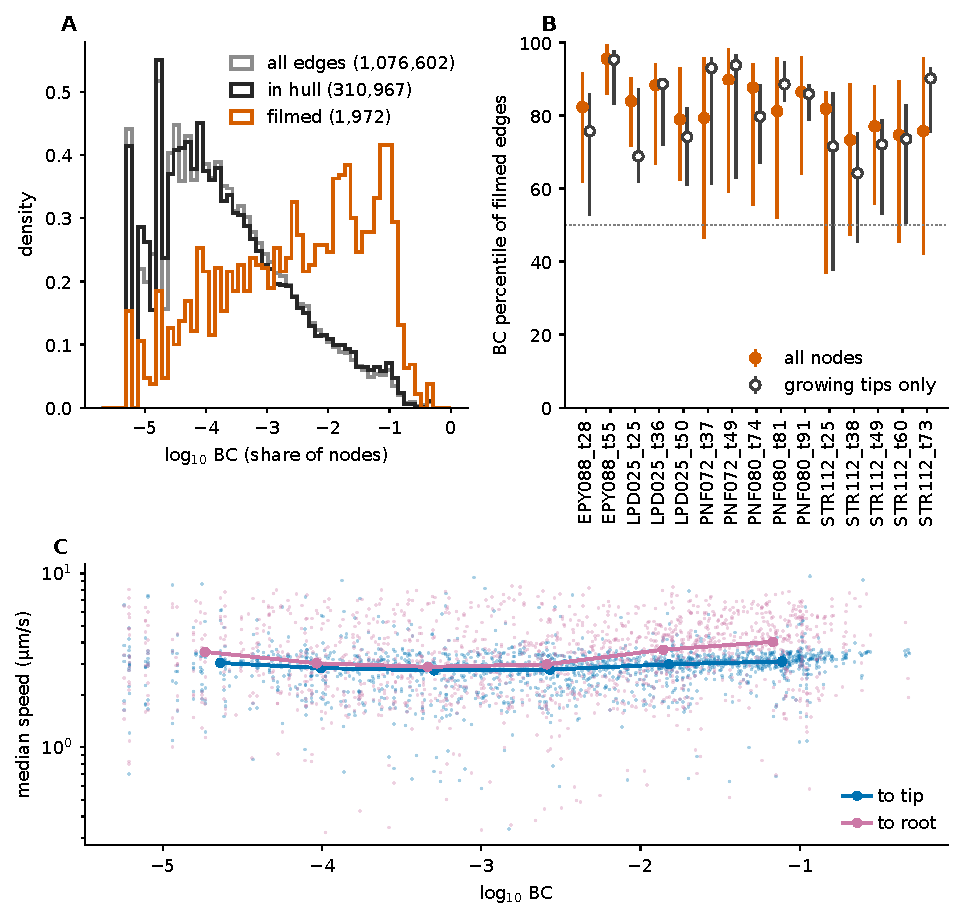
\includegraphics[width=\textwidth,keepaspectratio]{suppfig/figS_bc_selection.pdf}
\caption{[Caption to be written.]}
\label{fig:bc_selection}
\end{figure}

\namedsubsection{Tree-like edges and distance to the growing tips}{subsec:si_tree_tip}
% NOTE (10 Oct): section text to be written by Simon; cited from the Fig 1A caption (inset). Facts (transport_paper master, Working_notebooks/manuscript_figures/fig1.py, bridge_share_by_tip(); recomputed 10 Oct):
% NOTE (1, definition): an edge is tree-like when it is a bridge of the network graph (removing it disconnects the network; networkx bridges on the simple graph, degree-2 nodes dissolved), as in the model tables' `bridge` column; otherwise it lies on a loop. Methods, \nameref{subsec:dated_graph}, paragraph "Tree and loop edges", has the definition and a \todo for these bins.
% NOTE (2, edges): the filmed edges of the main model tables, 15 sessions (loop_density_curve.prepare_edges): 1,590 edges, 1,579 with a tip distance; tip distance = network distance to the nearest growing tip (d_tip, model_accuracy/features_edges.csv).
% NOTE (3, numbers, bins by tip distance in mm, n edges / % tree-like): <1: 86 / 39.5 %; 1-2: 201 / 20.4 %; 2-4: 438 / 10.5 %; 4-8: 568 / 10.7 %; >8: 286 / 14.3 % (main text: 40 % within 1 mm vs 11-14 % beyond 2 mm).
% NOTE (4, context): over all edges of the same networks 36 % are tree-like vs 15 % of the filmed edges (\nameref{subsec:si_video_selection}), so the filmed set under-samples tree-like edges.
% NOTE (5, open): a figure (share by tip distance, filmed vs all edges) if wanted; per-session spread.

\namedsubsection{Movement at the growing tips}{subsec:si_tips}
% NOTE (10 Oct): section text to be written by Simon; to be filled with more data later (Simon: does not lead to many conclusions yet). Sources: transport_paper explore/tip-diffusion (f4a8ba7, 37c25b3), manuscript/tip_diffusion_sketch.md; AMF_Transport#5; transport_paper#132 Q1.
% NOTE (1, streaks vs tip distance, bright-field, 654,711 streaks, 15 sessions): median to-tip streak duration 1.20 s within 0.5 mm of a tip vs 1.40-1.45 s beyond 1 mm; length 2.6 vs 4.2-4.5 um (shorter because slower, not shorter-lived). Per kymograph: median 38 moving streaks within 0.5 mm vs 118-149 beyond 2 mm; no moving streak in 20 % of kymographs within 1 mm vs 5-8 % beyond; static share of streaks 0.31 vs 0.02-0.04. Structure-tensor coherence flat (0.74-0.79). Many near-tip kymographs look clean but low-SNR (Simon). Caveats: detector minimum 15 frames (0.75 s) censors short or irregular movement; tip edges are short and counts are not length-normalised; streaks pooled without bootstrap.
% NOTE (2, videos with a tip in frame): the filmed positions rarely include a tip (selection, \nameref{subsec:si_video_selection}). In the first frames of the 96 videos nearest a tip (graph tip distance < 1.5 mm), 5 bright-field 20 fps videos have a free tip in frame (8 tip branches; STR2307A112, EPY2412A088, LPD2412A025, PNF2307A080, PNF2307A072); 2 more are 0.5 / 0.1 fps time-lapses.
% NOTE (3, kymographs traced by hand from the apex, figure below): within ~20 um of the apex movement is sparse and slow (~0.5-1 um/s, read by eye), in both directions in some branches, with stalls, small steps back and oscillations (period ~2 s, no net motion); much of the last 20 um is static; no long straight ~3 um/s streaks as elsewhere in the network. Low SNR; one video's apex uncertain.
% NOTE (4, open): more tip videos (targeted recordings, or a scan of the other video sets); particle tracking for an MSD; link to the near-tip slowdown (Fig 1E) and to the main-text qualifier 'no sign of random or back-and-forth movement'.

% -----------------------------------------------------------------------
% FIGURE: kymographs along tip branches, traced by hand from the apex
% Generated by transport_paper Working_notebooks/tip_crops_snellius.py (on Snellius) + tip_kymos_handtraced.py (explore/tip-diffusion 37c25b3)
% NOTE (10 Oct, caption is Simon's to write; facts): one row per tip branch; left: first frame with the trace (red) and the apex (cyan);
% middle: raw kymograph (x = distance from the apex along the hypha, um; y = time, s), mean over +/-3 px across the hypha;
% right: same with the time-mean removed (moving features only). 0.069 um/px, 20 fps; 10 s videos except PNF2307A072 (30 s).
% Rows: STR2307A112 2023-09-04 13:04:46 short and long branch; EPY2412A088 2025-01-22 12:12:01 branches a, b (trace off the hypha
% beyond ~15 um in b); LPD2412A025 2025-01-12 18:27:52 curled and right branch; PNF2307A080 2023-08-13 21:42:19; PNF2307A072
% 2023-08-10 14:35:58 (apex uncertain).
% -----------------------------------------------------------------------
\begin{figure}[hbt!]
\centering
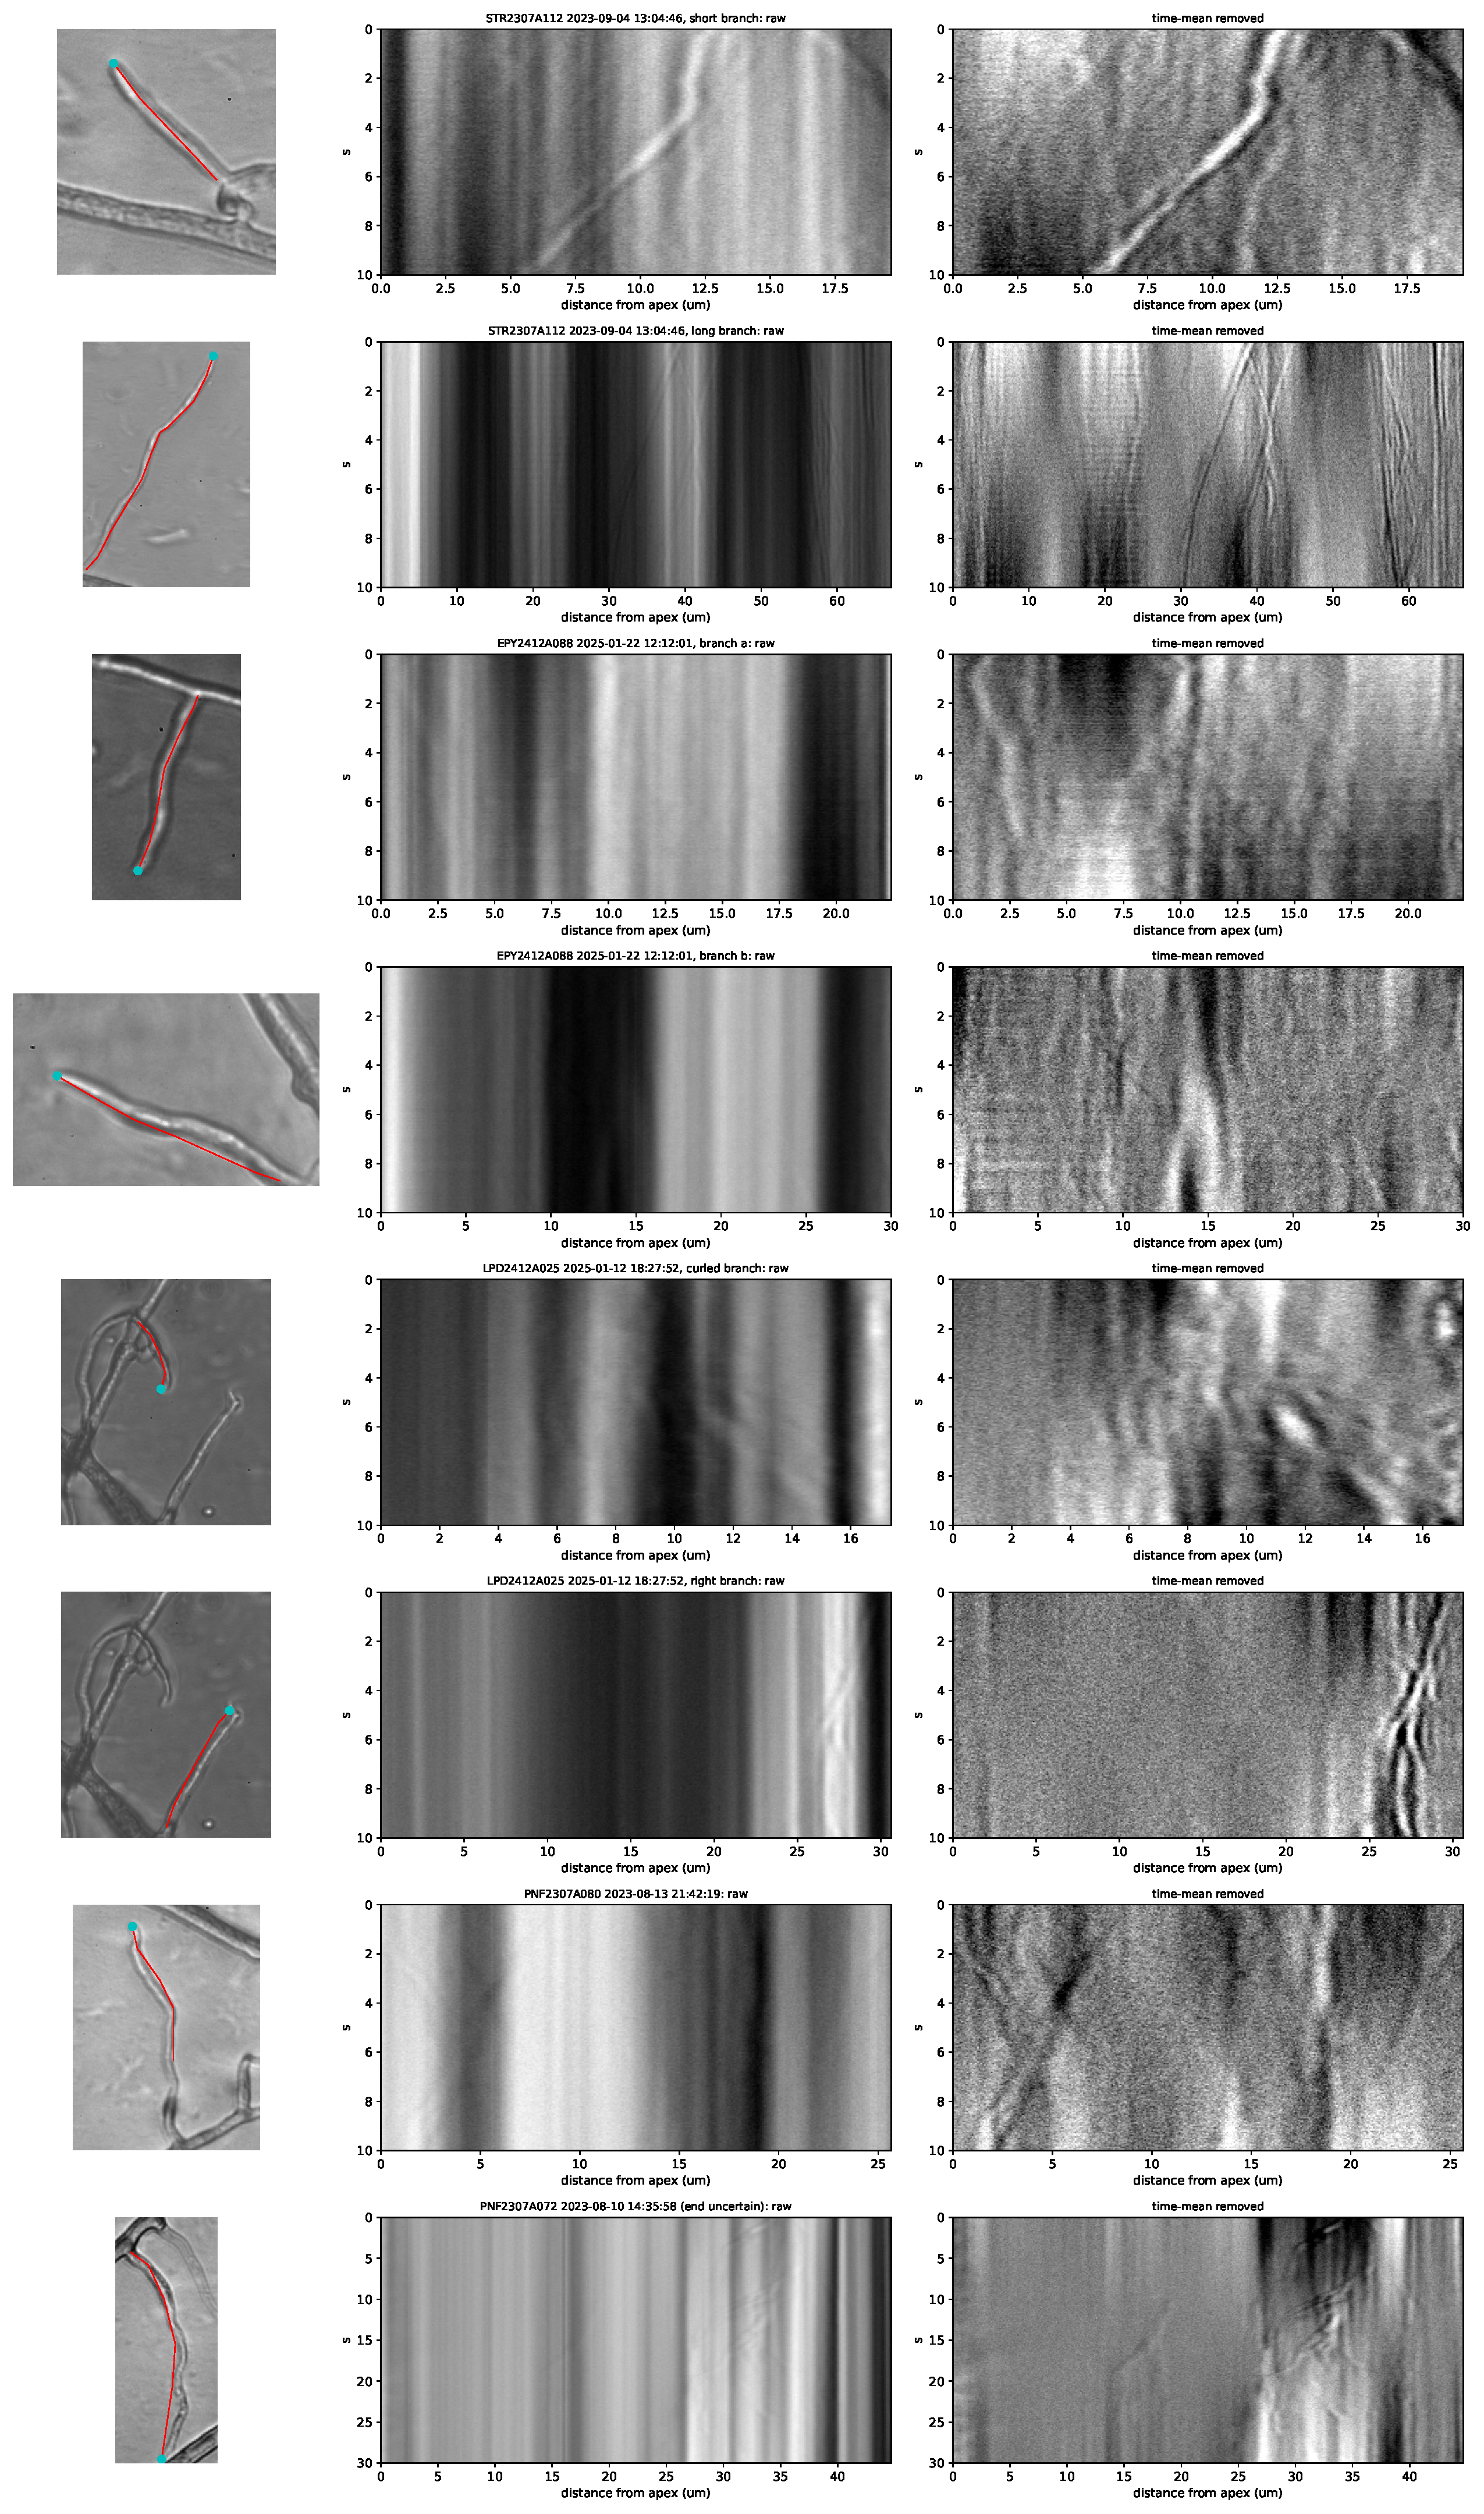
\includegraphics[width=\textwidth,height=0.9\textheight,keepaspectratio]{suppfig/figS_tip_kymos.pdf}
\caption{[Caption to be written.]}
\label{fig:tip_kymos}
\end{figure}

% -----------------------------------------------------------------------
% FIGURE: spread (IQR) of the speeds of all static-flow videos
% Referenced in main text (Results): "SI Fig.~\ref{fig:speed_iqr}"
% Generated by transport_paper Working_notebooks/manuscript_figures/figS_video_positions.py
% -----------------------------------------------------------------------
\begin{figure}[hbt!]
\centering
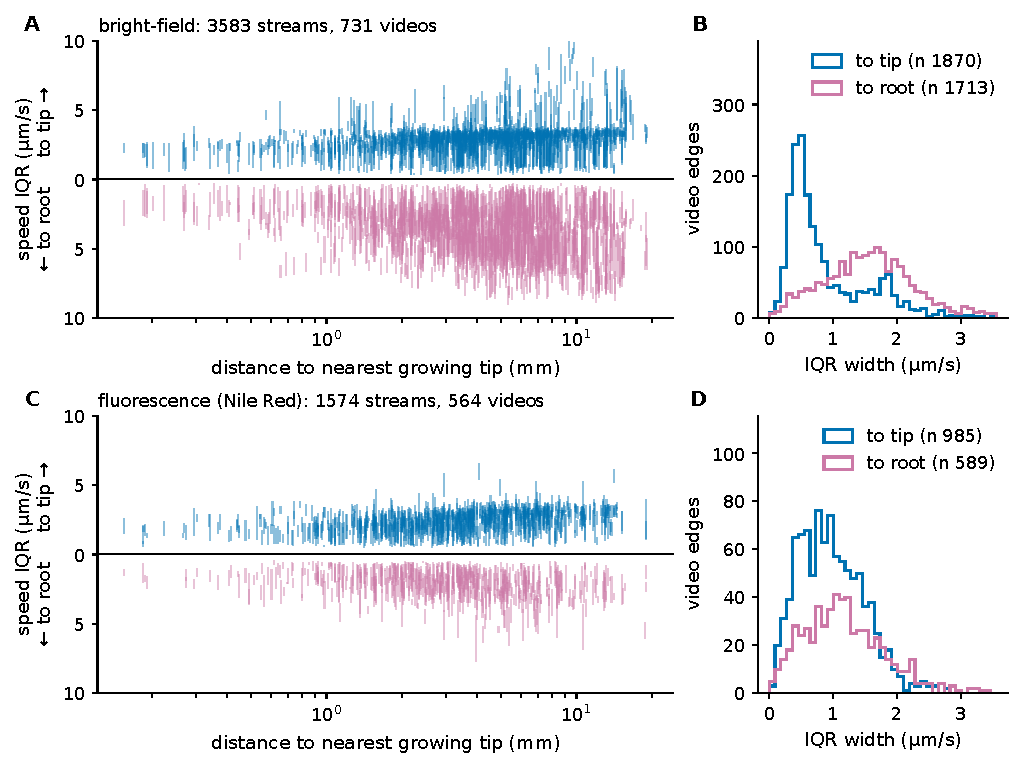
\includegraphics[width=\textwidth,keepaspectratio]{suppfig/FigS_video_positions_iqr.pdf}
\caption{\textbf{Spread of the speeds in the static-flow videos.}
Interquartile range (q25--q75) of the extracted to-tip and to-root speeds of each filmed hypha in the bright-field videos (3,583 hypha-direction streams from 731 videos; root-cut, section-cut and salt-shock videos excluded; directions with fewer than 5 streaks omitted).
Streaks count when they span at least 15 frames in bright-field (20~fps) and at least 5 frames in fluorescence (1--2~fps).
\textbf{(A, B)} Bright-field.
\textbf{(C, D)} Fluorescence (Nile Red) videos, same rules and axis ranges (2,385 streams from 625 videos).
\textbf{(A, C)} Bars against distance to the nearest growing tip, to-tip up (blue) and to-root down (pink).
\textbf{(B, D)} Distribution of the IQR widths.
The median IQR is 0.63~$\mu$m/s to tip and 1.58~$\mu$m/s to root in bright-field, and 1.07~$\mu$m/s to tip and 1.22~$\mu$m/s to root in fluorescence.}
\label{fig:speed_iqr}
\end{figure}
% NOTE (10 Oct, IQRs of censored speeds (transport_paper#132 comment 6088415445; feat/fl-numbers-limits 8391a7e, manuscript/fl_numbers_limits.md)): median IQR to tip / to root, streaks < 5 um/s in both modes: bright-field 0.62 / 1.25, Nile Red 1.06 / 1.17 (directions with q75 < 5: 0.60 / 1.41 vs 1.07 / 1.18). So the bright-field to-root spread drops toward Nile Red once truncated, the to-tip one does not. Nile Red directions have a median of 14 streaks vs 87 in bright-field.

% -----------------------------------------------------------------------
% FIGURE: to-tip against to-root speed per edge, fluorescence vs bright-field
% Same plot as Fig.~\ref{fig:asymmetries}A (fig2.py, draw_arm_density), fed with the
% fluorescence data. Numbers from the min_frames=5 fluorescence streaks (7 Oct).
% Generated by transport_paper Working_notebooks/manuscript_figures/figS_video_positions.py
% -----------------------------------------------------------------------
\begin{figure}[hbt!]
\centering
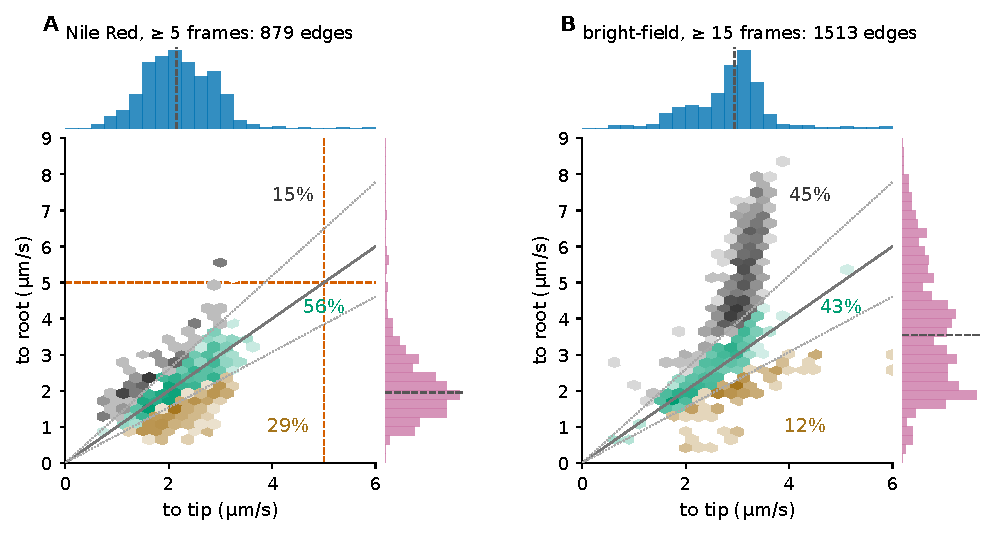
\includegraphics[width=\textwidth,keepaspectratio]{suppfig/figS_fl_forward_backward_density.pdf}
\caption{\textbf{To-tip against to-root speeds in fluorescence and bright-field.}
Density plots of the absolute to-tip speed against the absolute to-root speed at the same location, drawn as in Fig.~\ref{fig:asymmetries}A, for \textbf{(A)} the Nile Red fluorescence videos and \textbf{(B)} the bright-field videos (static-flow videos only; streaks of at least 5 frames in fluorescence and 15 frames in bright-field; 879 fluorescence and 1,513 bright-field edges with both directions, as given above each panel).
Median speeds are 2.15~$\mu$m/s to tip and 1.96~$\mu$m/s to root in fluorescence, against 2.95 and 3.55~$\mu$m/s in bright-field.
Marginal histograms with medians (dashed); hexes are coloured by their relation to 1:1 within a factor 1.3 (to-root faster, similar, to-tip faster) with the share of edges in each category.
Fluorescence videos were imaged at 1 or 2~fps (10 or 20 frames) against 20~fps for bright-field.
The dashed lines in A at 5~$\mu$m/s mark a rough estimate of where under-sampling could start, assuming a feature spacing of about 5~$\mu$m in the Nile Red kymographs (2.5~$\mu$m per frame at 2~fps); this spacing was not measured.}
\label{fig:fl_forward_backward}
\end{figure}
% NOTE (10 Oct (transport_paper#132 comment 6088415445; feat/fl-numbers-limits 8391a7e, manuscript/fl_numbers_limits.md)): caption medians 2.15 / 1.96 vs 2.95 / 3.55 are full-range streak medians (Nile Red censored above ~5). Per-pixel (2 fps, >= 100 px): Nile Red 2.42 / 2.20 (595 edges) vs bright-field 2.74 / 2.91 (1,513); paired 532 edges 2.38 / 2.15 vs 2.56 / 2.46. The dashed 5 um/s line stands, but its rationale ('rough estimate, feature spacing') is superseded: the limit is measured (half-peak 4.9 um/s at 2 fps, 4.7-5.1 at 1 fps; fig:fl_detection_limit).

% -----------------------------------------------------------------------
% FIGURE: detection of fluorescence streaks against speed
% Referenced in Methods (subsec:fl_detection_limit): "SI Fig.~\ref{fig:fl_detection_limit}"
% Generated by transport_paper Working_notebooks/manuscript_figures/figS_fl_detection_limit.py
% Numbers: transport_paper fig_outputs/synthetic_streak_ceiling/ceilings.csv, bf_subsampled_fl/efficiency.csv,
% pixel_noise_control/speed_summary.csv (notes synthetic_streak_ceiling.md, bf_subsampled_fl_efficiency.md,
% pixel_noise_control.md, 7 Oct).
% -----------------------------------------------------------------------
\begin{figure}[hbt!]
\centering
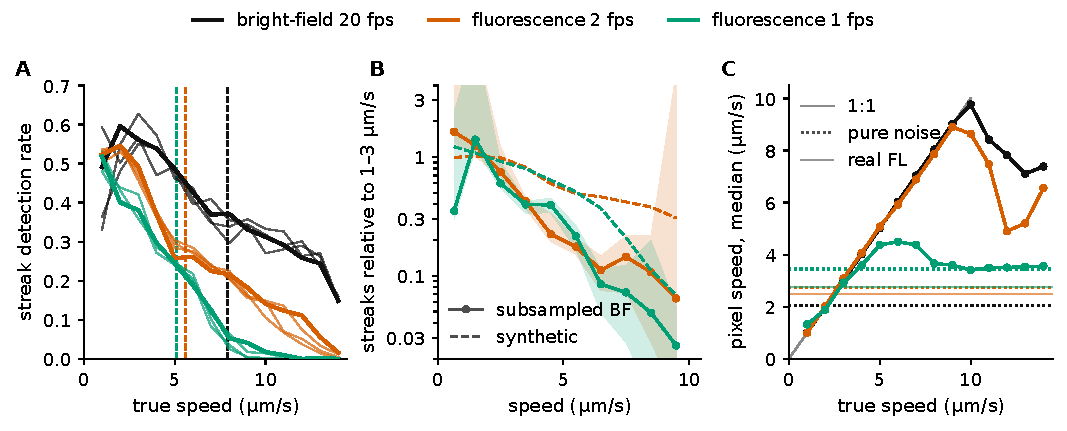
\includegraphics[width=\textwidth,keepaspectratio]{suppfig/figS_fl_detection_limit.pdf}
\caption{\textbf{Detection of fluorescence streaks against speed.}
Bright-field at 20~fps (black), fluorescence at 2~fps (orange) and at 1~fps (green), in all panels.
\textbf{(A)} Fraction of synthetic particles found as a streak against their true speed, for synthetic kymographs passed through the same normalisation, resampling, orientation filter and streak detection as the data (particles of 0.8~$\mu$m FWHM moving in both directions, calibrated density, automatic filter centre; streaks of at least 15 frames in bright-field and 5 in fluorescence).
Thick lines: exposure 0.9 of the frame period, as in the experiments; thin lines: exposure 0.01, 0.1 and 0.5, which coincide with it.
The detection rate falls to half its low-speed peak at 10.7~$\mu$m/s in bright-field, 4.9~$\mu$m/s at 2~fps and 4.7 to 5.1~$\mu$m/s at 1~fps (5 or 8 frames minimum).
Dashed vertical lines: 99th percentile of the measured streak speeds in each mode (7.9, 5.6 and 5.1~$\mu$m/s).
\textbf{(B)} Bright-field kymographs (1,296 kymographs, three plates) averaged and decimated to 2 and 1~fps and run through the fluorescence settings: streaks found per bright-field streak in the same 1~$\mu$m/s speed bin, relative to the mean of the 1 to 3~$\mu$m/s bins (solid, with the plate-then-kymograph bootstrap 95\% interval, cut at the axis limits; bins with fewer than 100 bright-field streaks omitted; logarithmic axis).
At 5 to 6~$\mu$m/s this is 0.18 at 2~fps and 0.22 at 1~fps (0.050 and 0.030 streaks per bright-field streak), against 0.49 and 0.51 for the synthetic efficiency of A at the same bins (dashed).
\textbf{(C)} Speed returned by the orientation filter per pixel, as the median over kymographs of the per-direction pixel median, against the true speed of synthetic particles moving in one direction at the calibrated density; grey line 1:1.
Dotted lines: the same statistic on pure-noise kymographs; thin solid lines: the median over the measured fluorescence directions.
At 2~fps the pixel median stays within 0.3~$\mu$m/s of the true speed up to 9~$\mu$m/s, at 1~fps it saturates at 4.4 to 4.5~$\mu$m/s (true speeds 5 to 7~$\mu$m/s) and falls back to the noise level from 8~$\mu$m/s.
The synthetic data are idealised: white pixel-independent noise, constant-speed Gaussian particles, no static structure or bleaching, and a weak calibration of density and noise, to which the limit in A is most sensitive.
In B the pipeline normalisation was applied to the 20~fps video before averaging and decimation, and the emulation was not checked against raw videos.}
\label{fig:fl_detection_limit}
\end{figure}
% NOTE (10 Oct (transport_paper#132 comment 6088415445; feat/fl-numbers-limits 8391a7e, manuscript/fl_numbers_limits.md)): the dashed 99th-percentile lines (7.9 / 5.6 / 5.1 um/s) come from the 8-frame production tables; for the 5-frame streaks the paper plots they are 8.1 (bright-field) / 6.1 (2 fps) / 5.3 (1 fps); figS_fl_detection_limit.py hard-codes the old values (same values in Methods L151). Caption C says pixel median valid 'up to 9 um/s', Methods says '8 to 9'.

% -----------------------------------------------------------------------
% FIGURE: to-tip against to-root speed per filmed hypha, coloured by distance to the nearest growing tip
% Generated by transport_paper Working_notebooks/manuscript_figures/figS_tip_root_scatter.py (161cf3f)
% NOTE (7 Oct, caption is Simon's to write; facts): one dot per video edge (one video of one hypha) with both streams
% measured, x/y = median absolute streak speed of each stream; colour = network distance to the nearest growing tip
% (mm, log scale 0.1-20, clipped; open grey = no tip distance); line = identity; axes cut at the 99.5th percentile (8 um/s).
% Same video edges, stream assignment and tip distance as the IQR figure (figS_video_positions); fluorescence = 5-frame
% streaks, bright-field = 15. (A) bright-field: 1,619 video edges (10 without tip distance), medians to tip 2.96 / to root
% 3.43 um/s, Spearman rho tip-root 0.64, to-root vs distance 0.25, to-tip vs distance 0.28. (B) Nile Red: 888 (6),
% 2.13 / 1.96 um/s, rho 0.53, 0.31, 0.29. Read: near tips the dots sit on the diagonal at ~2 um/s; both fast arms
% (to-root up to 8 um/s, and the horizontal fast to-tip arm at 4-8 um/s) are far from tips.
% NOTE (7 Oct, caveat for B, from the 'Fluorescence slow bias?' session, transport_paper#132): Nile Red streak speeds
% are censored above ~5 um/s (10-20 frames per video; half-peak ceiling 4.7-5.1 um/s vs 10.7 in bright-field). The
% absence of fast Nile Red dots in B is therefore not evidence that the fast streams carry no lipid; do not compare A and
% B above 5 um/s. Forward model: no evidence that the fast to-root stream is unstained, a twofold deficit not excluded.
% NOTE (7 Oct, later, SUPERSEDES the 'no evidence ... unstained' clause above; same session, transport_paper#132): per-pixel
% speeds (valid to ~8-9 um/s at 2 fps with >= ~100 pixels; not at 1 fps) show the detection limit explains only part of
% the smaller fast to-root branch in Nile Red. On 532 edges with both modes, to-root >1.3x faster on 39 % in bright-field
% vs 21 % in fluorescence (2 fps pixel medians 2.42 tip / 2.20 root um/s). Why less of the fast return is stained is open.
% -----------------------------------------------------------------------
\begin{figure}[hbt!]
\centering
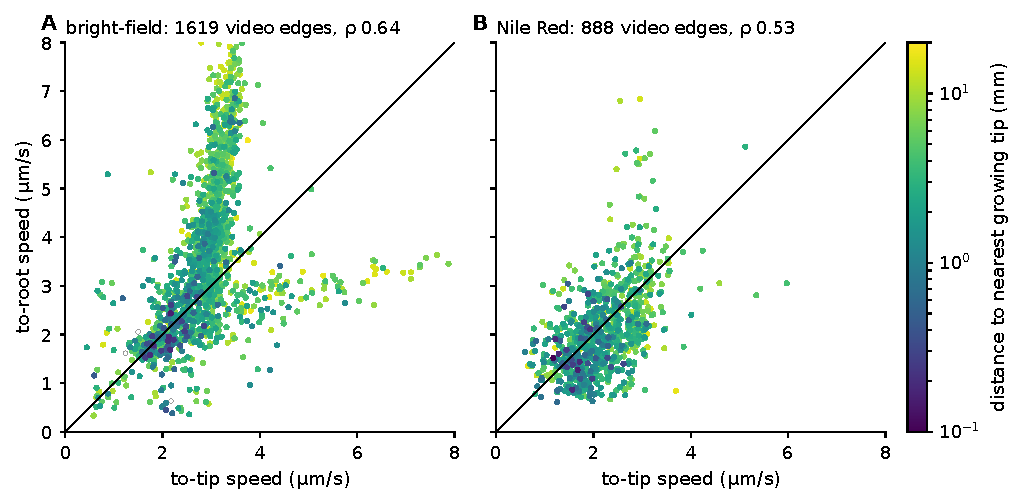
\includegraphics[width=\textwidth,keepaspectratio]{suppfig/figS_tip_root_scatter.pdf}
\caption{[Caption to be written.]}
\label{fig:tip_root_scatter}
\end{figure}
% NOTE (10 Oct, supersedes the Nile Red numbers in the note above (transport_paper#132 comment 6088415445; feat/fl-numbers-limits 8391a7e, manuscript/fl_numbers_limits.md)): panel B is streak medians, censored above ~5 um/s. Per-pixel at 2 fps: Nile Red 608 video edges, medians 2.40 / 2.20, rho 0.65; bright-field pixels 2,194 video edges, 2.76 / 2.73, rho 0.66.

% -----------------------------------------------------------------------
% FIGURE: osmotic shock, examples, response against osmolarity, Nile Red
% Referenced in main text (Results, osmotic paragraph): "SI Fig.~\ref{fig:salt_shock}D"
% Generated by transport_paper Working_notebooks/figure3/salt_shock_me.py (figS_salt_shock)
% -----------------------------------------------------------------------
\begin{figure}[hbt!]
\centering
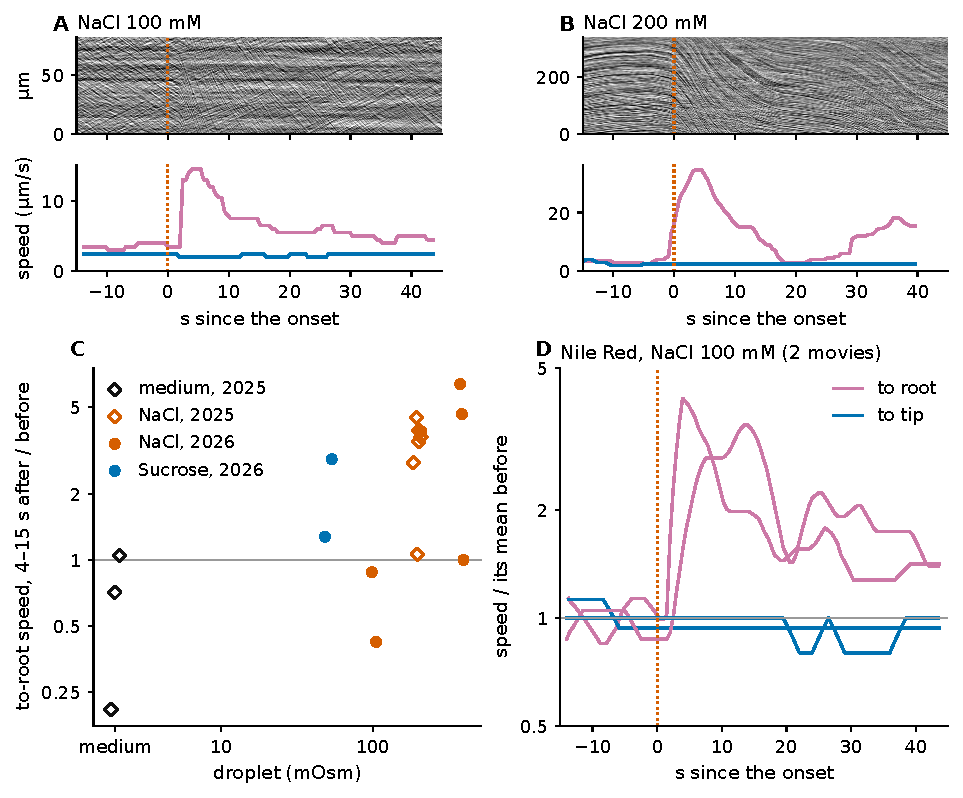
\includegraphics[width=0.9\textwidth,keepaspectratio]{suppfig/figS_salt_shock.pdf}
\caption{\textbf{Osmotic shock: examples, dependence on the droplet and lipid movement.}
\textbf{(A, B)} Two example kymographs after a drop of NaCl solution (100 mM and 200 mM) with the speed of the two streams below, to root (pink) and to tip (blue); dotted line: onset of the response.
\textbf{(C)} Change in the to-root speed, 4--15~s after the drop divided by $-10$ to $-1$~s before it, against the osmolarity of the droplet (medium-like drops at the left; NaCl in 2025 and 2026, sucrose in 2026).
\textbf{(D)} The two Nile Red fluorescence movies of NaCl 100 mM drops: speed to root (pink) and to tip (blue) divided by its mean before the drop.
The lipids, like the bright-field flow, keep their to-tip speed while the to-root speed rises.}
\label{fig:salt_shock}
\end{figure}

\clearpage

% -----------------------------------------------------------------------
% FIGURE S2
% Actively referenced in main text (lines 93, 97, 99, 144, 150):
%   "Fig. SI\ref{fig:carbonflow}b/d/e/f"
% Content: hydraulic (growth-induced mass-flow) model predictions vs
%          measurements; lipid volume-fraction spatial profile.
% Subfigures mentioned in text: b (predicted motor direction),
%   c (direction agreement, commented), d (speed comparison),
%   e (speed histogram), f (lipid volume fraction along hypha).
% -----------------------------------------------------------------------
\begin{figure}[hbt!]
\centering
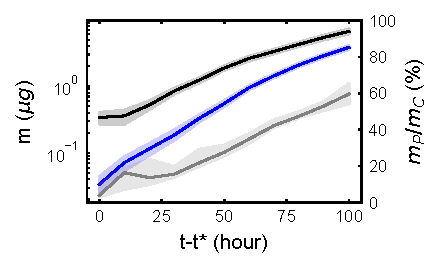
\includegraphics[width=\textwidth]{suppfig/FigS2.pdf} % WRONG FILE (checked 2 Oct): shows mass (ug) and m_P/m_C over t-t* (one panel), not the caption's 6 hydraulic panels. Candidate: transport_paper manuscript/figures/figS_net_flux.pdf (A: net lumen speed ~0.1-1 um/s, i.e. growth-driven flow alone is far below the measured 2-8 um/s); panels differ, caption needs rewriting.
\caption{\textbf{Growth-induced mass-flow model cannot explain observed speeds.}
\textbf{(A)} TODO.
\textbf{(B)} Predicted lipid flux direction from hydraulic minimisation.
Color indicates direction.
\textbf{(C)} Comparison of estimated and observed flux directions.
Percentage of agreement as a function of exclusion radius.
\textbf{(D)} Measured speed vs hydraulic model speed for all edges.
Model does not reproduce observed speeds.
\textbf{(E)} Histogram of absolute hydraulic speeds across whole network compared to measured bright-field speeds.
\textbf{(F)} Lipid volume fraction $\theta$ estimated from growth flux, plotted against distance from the hyphal tip.
}
\label{fig:carbonflow}
\end{figure}

\clearpage

% -----------------------------------------------------------------------
% FIGURE S3
% Referenced in commented-out text (line 64):
%   "SI Fig.\ref{fig:replicates}"
% Content: speed asymmetry dataset from 6 developmental time-points
%          across 2 plates, ~2000 edges total.
% Uncomment the section in main text (line 64) when this figure is ready.
% -----------------------------------------------------------------------
\begin{figure}[hbt!]
\centering
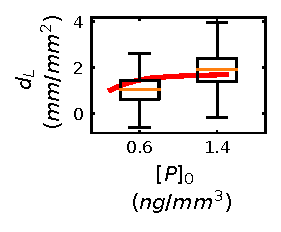
\includegraphics[width=\textwidth]{suppfig/FigS3.pdf} % WRONG FILE (checked 2 Oct): shows d_L against [P]_0 (boxplots), not speed asymmetry. No current replacement: needs a per-plate/per-session version of Fig 2A (to-root vs to-tip). figS_measurement_map.pdf shows where edges were measured, not the asymmetry.
\caption{\textbf{Speed asymmetry replicated across developmental time-points.}
\textbf{(A)} TODO: overview of all ~2000 measured edges across 6 time-points and 2 plates.
\textbf{(B)} TODO.
}
\label{fig:replicates}
\end{figure}

\clearpage

% -----------------------------------------------------------------------
% FIGURE S4
% Referenced in commented-out text (lines 83, 83):
%   "Figure \ref{fig:lipid_flows}d"  /  "SI Fig showing all replicates"
% Content: directional lipid kymographs and Fourier-filtered versions
%          showing net tipward flux; all replicate panels.
% Uncomment the section in main text (lines 82-84) when ready.
% -----------------------------------------------------------------------
\begin{figure}[hbt!]
\centering
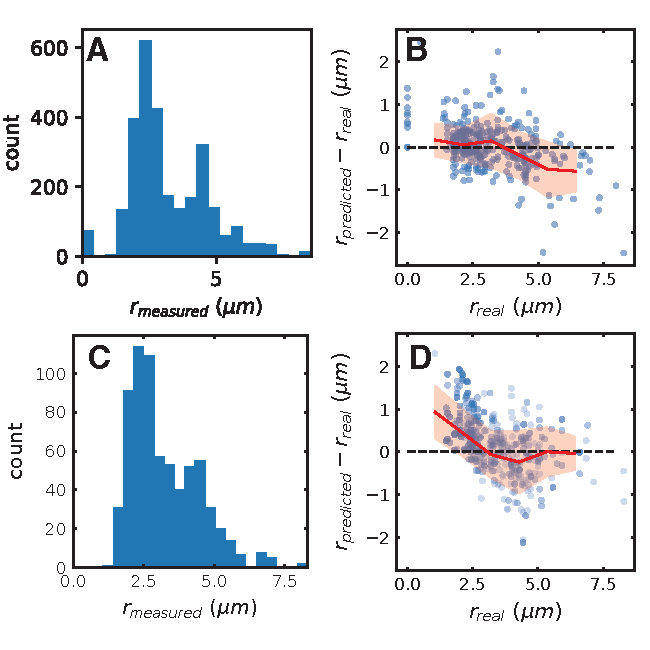
\includegraphics[width=\textwidth]{suppfig/FigS4.pdf} % WRONG FILE (checked 2 Oct): shows measured-radius histograms and r_predicted - r_real, not lipid direction. Closest: transport_paper manuscript/figures/figS_lipid_bias.pdf (per-plate share strongly to tip, fluorescence vs brightfield, vs tip distance); kymograph panels are already Fig 2D; caption needs rewriting.
\caption{\textbf{Lipid movement is predominantly tipward across all replicates.}
\textbf{(A)} TODO.
\textbf{(B)} TODO.
\textbf{(C)} TODO.
\textbf{(D)} Aggregate net flux direction in fluorescence (red) and bright-field (black) for all measured trails.
}
\label{fig:lipid_flows}
\end{figure}

\clearpage

% -----------------------------------------------------------------------
% FIGURE S5
% Referenced in commented-out text (line 165):
%   "Fig. \ref{fig:hydraulic_proportionality}b"
% Content: model prediction of C/P exchange proportionality emerging
%          from lipid-induced backflow.
% Uncomment the paragraph in main text (lines 164-167) when ready.
% -----------------------------------------------------------------------
\begin{figure}[hbt!]
\centering
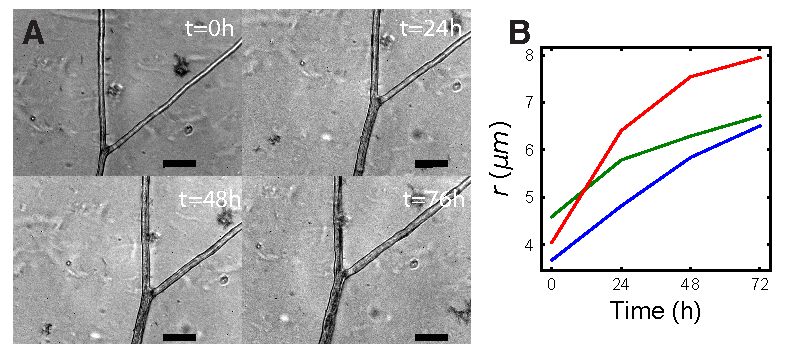
\includegraphics[width=\textwidth]{suppfig/FigS5.pdf} % WRONG FILE (checked 2 Oct): shows hyphae thickening over 72 h (images, r vs time), not C/P exchange. No current replacement in transport_paper.
\caption{\textbf{Lipid-backflow model predicts proportional C/P exchange.}
\textbf{(A)} TODO.
\textbf{(B)} Carbon flux from plant vs phosphorus flux from fungal colony under the backflow model, showing proportional scaling.
}
\label{fig:hydraulic_proportionality}
\end{figure}

\clearpage

% -----------------------------------------------------------------------
% ADDITIONAL FIGURES (not yet labelled in main text)
% Assign \label and add \ref in main text when ready to use.
% -----------------------------------------------------------------------

\begin{figure}[hbt!]
\centering
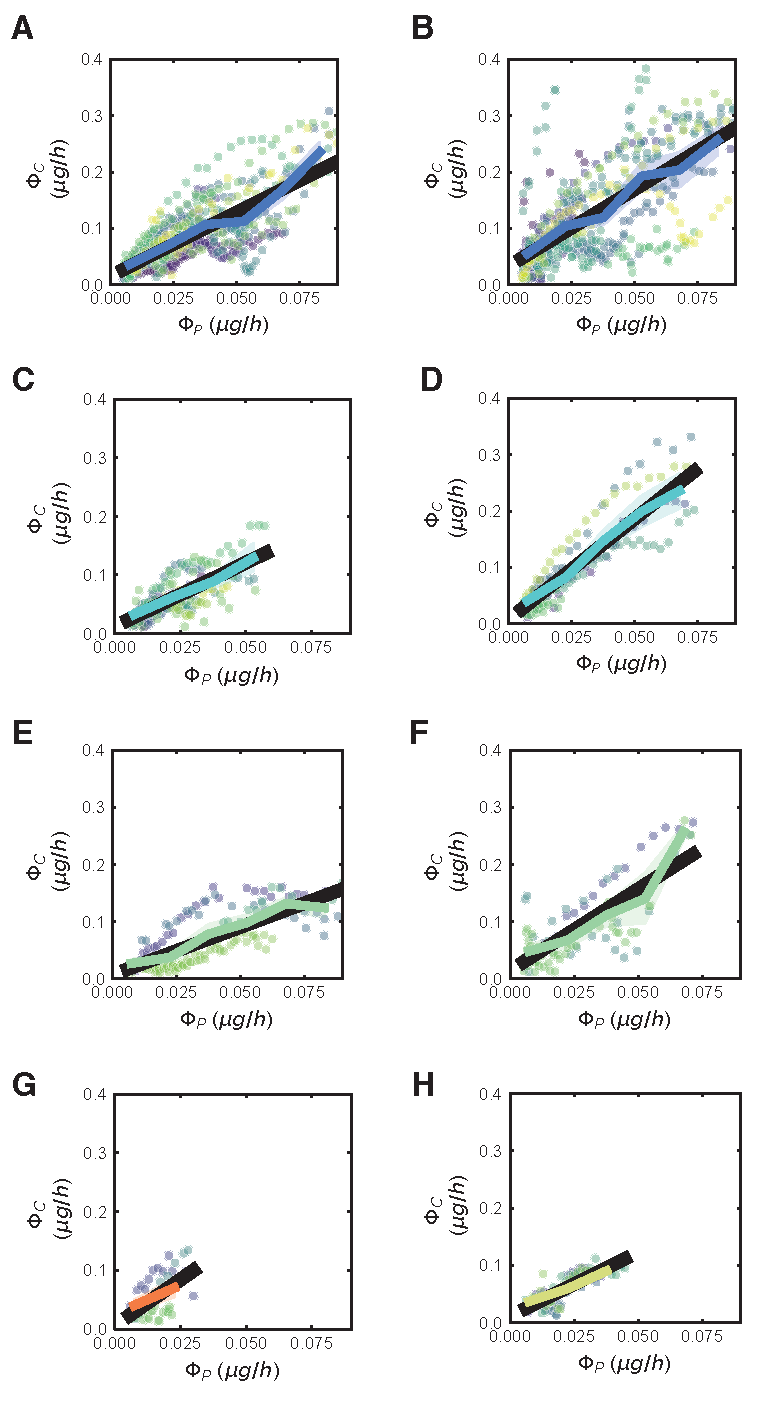
\includegraphics[width=\textwidth,height=0.8\textheight,keepaspectratio]{suppfig/FigS_replicate_4A.pdf}
% TRIAGED 2 Oct: Phi_C vs Phi_P (ug/h), 8 replicates A-H with linear fits: the C-P proportionality data (Bisot et al.). Goes with transport_paper#128 (C/P framing): keep if that framing stays, or cite if published.
\caption{\textbf{TODO: Replicate 4A.}
TODO caption.}
% \label{fig:replicate_4A}
\end{figure}

\clearpage

\begin{figure}[hbt!]
\centering
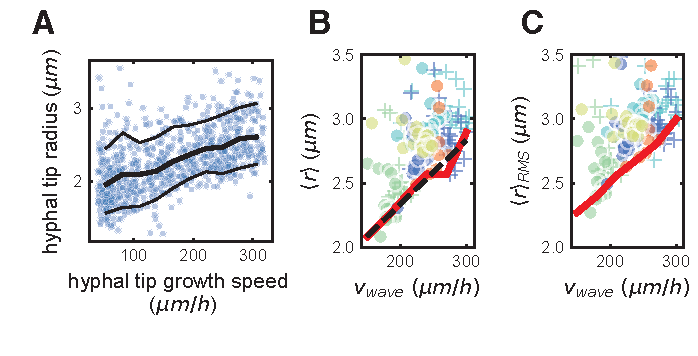
\includegraphics[width=\textwidth]{suppfig/FigSradius_speed.pdf}
% TRIAGED 2 Oct: tip radius vs tip growth speed, <r> vs travelling-wave speed: from the travelling-wave work (Oyarte Galvez 2025), not transport. Suggest drop unless a width-speed argument needs it (transport_paper#129).
\caption{\textbf{TODO: Radius vs speed.}
TODO caption.}
% \label{fig:radius_speed}
\end{figure}

\clearpage

\begin{figure}[hbt!]
\centering
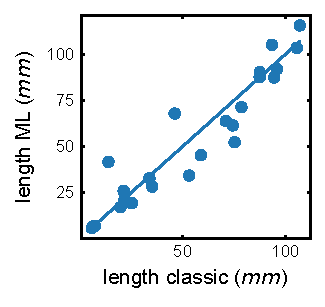
\includegraphics[width=\textwidth]{suppfig/FigureComparison.pdf}
% TRIAGED 2 Oct: network length, ML vs classic segmentation (~25 points): an older segmentation check. Suggest replace with transport_paper manuscript/figures/S_segmenter.png (current pipeline) or drop (transport_paper#129).
\caption{\textbf{TODO: Comparison figure.}
TODO caption.}
% \label{fig:comparison}
\end{figure}

\clearpage

\begin{figure}[hbt!]
\centering
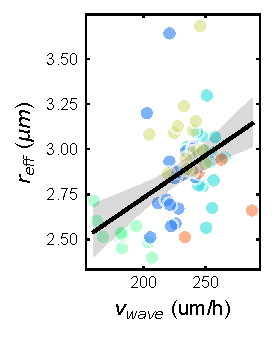
\includegraphics[width=\textwidth]{suppfig/FigureSRspeeddrag.pdf}
% TRIAGED 2 Oct: r_eff vs travelling-wave speed: travelling-wave work, not transport. Suggest drop (transport_paper#129).
\caption{\textbf{TODO: Speed-drag figure.}
TODO caption.}
% \label{fig:speed_drag}
\end{figure}

\clearpage

\begin{figure}[hbt!]
\centering
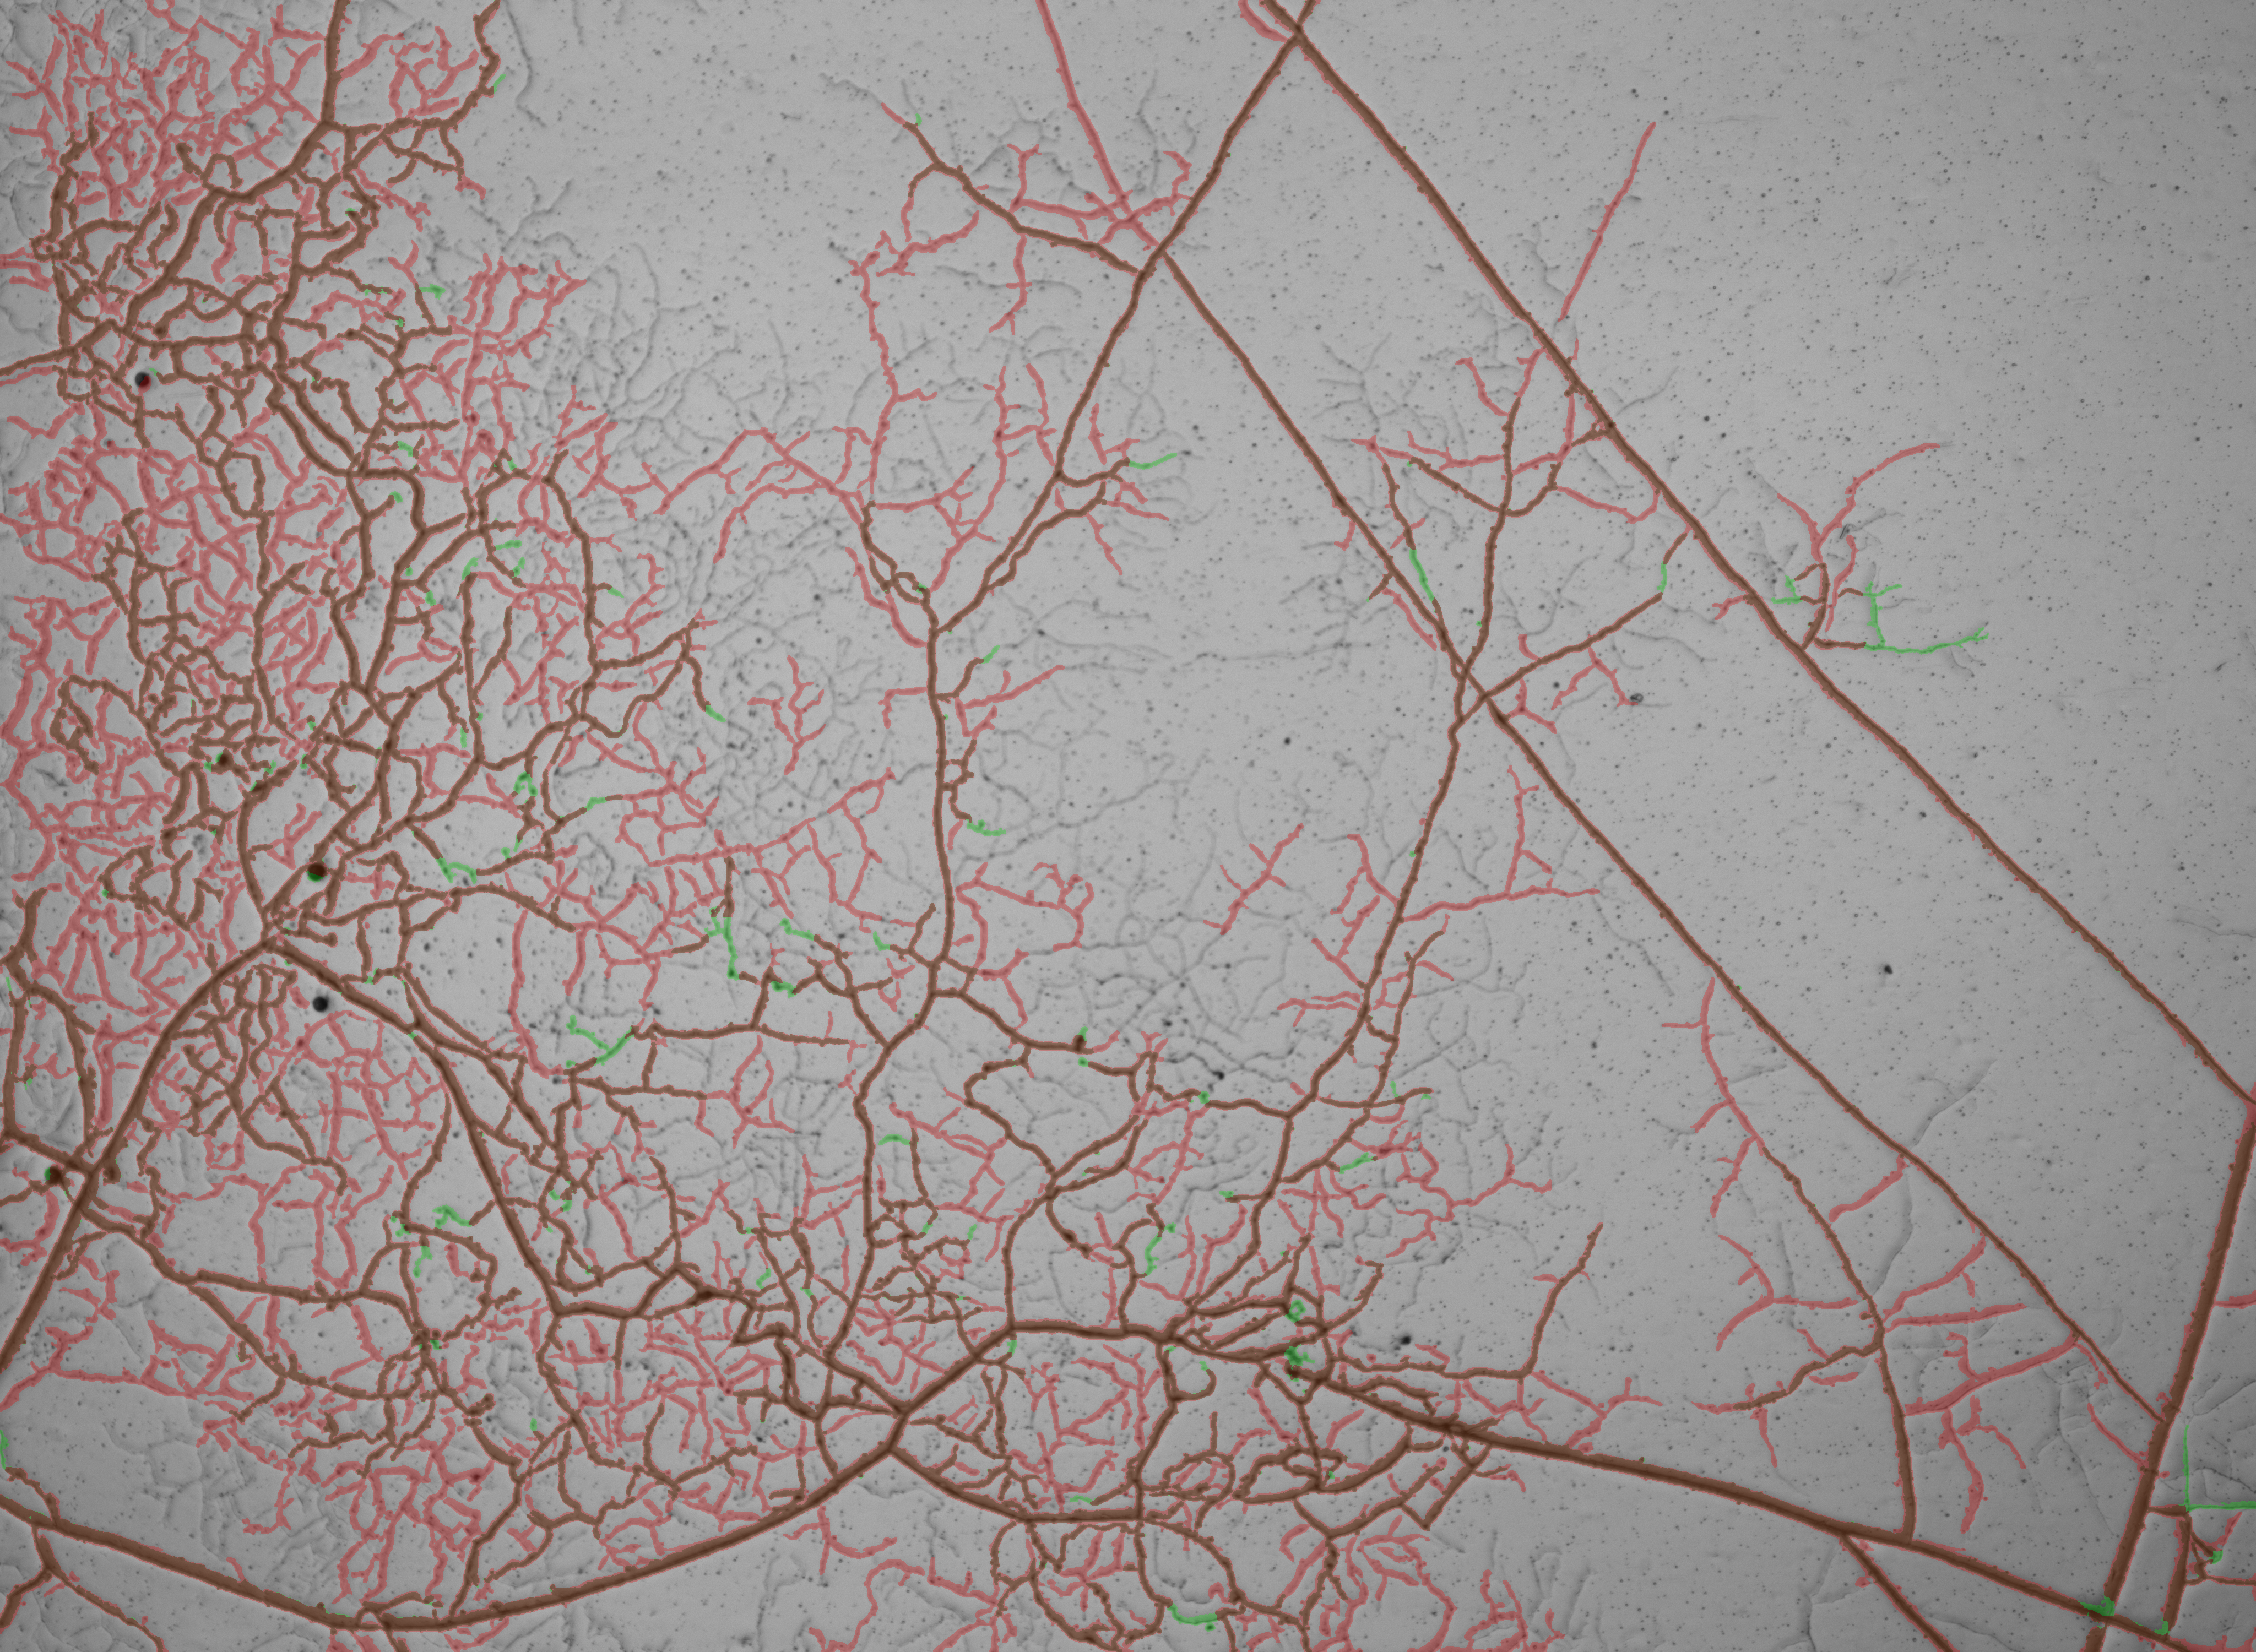
\includegraphics[width=0.9\textwidth]{suppfig/symbiotic-hard-comparison.png}
% TRIAGED 2 Oct: dense network with a segmentation overlay: an older segmentation check. Suggest replace with the current pipeline SI figures (S_segmenter, S_graph_repair) or drop (transport_paper#129).
\caption{\textbf{TODO: Symbiotic hard comparison.}
TODO caption.}
% \label{fig:symbiotic_comparison}
\end{figure}

% %  CONFIGURE NEW SINGLE-PAGE FORMAT 

\onecolumn % go back to one column
\fancyhead{} % make sure we get no headers
\renewcommand{\floatpagefraction}{0.1}
\lfoot[\bSupInf]{\dAuthor}
\rfoot[\dAuthor]{\cSupInf}
\newpage

\captionsetup*{format=largeformat} % make figure legend slightly larger than in the paper
\setcounter{figure}{0} % reset figure counter for Supplementary Video Figures
%\setcounter{page}{1} % reset page count
\makeatletter 
\renewcommand{\thefigure}{SV\@arabic\c@figure} % make Figure legend start with Figure S
\makeatother

%  MAIN TEXT 
\newpage
\section*{Supplementary Videos}

\begin{SCfigure*}[50][!ht]
\includegraphics[width=0.5\linewidth]{Figures/temp.png}
\caption{\textbf{This is a video of a lysosome.}\\
A typical caption would go here. We use a thumbnail version of the video file as the figure.\\
Time, seconds. Scale bar, \SI{10}{\micro\meter}.}
\label{videosupp:lysosome}
\end{SCfigure*}
% %  CONFIGURE NEW SINGLE-PAGE FORMAT 

\onecolumn % go back to one column
\fancyhead{} % make sure we get no headers
\renewcommand{\floatpagefraction}{0.1}
\lfoot[\bSupInf]{\dAuthor}
\rfoot[\dAuthor]{\cSupInf}
\newpage

\captionsetup*{format=largeformat} % make legend slightly larger than in the paper
\setcounter{table}{0} % reset table counter for Supplementary Video Figures
%\setcounter{page}{1} % reset page count
\makeatletter 
\renewcommand{\thetable}{S\@arabic\c@table} % make Table legend start with Table S
\makeatother

%  MAIN TEXT 
\newpage
\section*{Supplementary Tables}

\bigskip

\begin{table}[!h]
    \centering
    \small
    \begin{tabular}{p{3cm}|p{2.2cm} p{2.2cm} p{2.2cm} p{2.2cm} p{2.2cm}}
        Movie & US Release Date & Director & Screenwriter(s) & Story by & Producer\\
        \hline
        Episode IV – A New Hope & May 25, 1977 & \multicolumn{3}{c}{George Lucas} & Gary Kurtz\\
        Episode V – The Empire Strikes Back & May 21, 1980 & Irvin Kershner & Leigh Brackett and Lawrence Kasdan & George Lucas & Gary Kurtz\\
        Episode VI – Return of the Jedi & May 25, 1983 & Richard Marquand & Lawrence Kasdan and George Lucas & George Lucas & Howard Kazanjian\\
    \end{tabular}
    \caption{\textbf{Original ``Star Wars'' Trilogy}\\
    Extracted from \url{https://en.wikipedia.org/wiki/List_of_Star_Wars_films}.}
    \label{supptab:st1}
\end{table}





\end{document}